%!TeX root = 1-screening
\documentclass[main.tex]{subfiles}

\begin{document}

\chapter{High-throughput Computational Screening of Nanoporous Materials}
\vspace*{-1\baselineskip}

\section{Nanoporous Materials}

\subsection{Introduction and Concepts}

\subsubsection{Adsorption isotherms and geometrical Descriptors}

%General introduction
Nanoporous materials are defined as materials with a nanoscale structure constituted by pores and cavities, which some are connected by a network of channels. These pores can be empty or filled with a variety of substances called adsorbates. By adhering molecules from a liquid or gas phase into the internal surfaces of the material, we can use it in various applications such as gas separation and purification,\cite{Li_2009,Lagorsse_2007} energy storage and conversion,\cite{Morris_2008,Qiu_2020} heterogeneous catalysis\cite{Bell_2003,Singh_2019,Pascanu_2019} drug delivery,\cite{Della_Rocca_2011,Bernini_2014} or sensing.\cite{Breslin_1976} By designing the chemical nature, size, shape and distribution of the pores, we can tailor the physicochemical properties to the targeted application.\cite{Yan_2020}

%adsorption
The process of adhering particles or molecules on surfaces is called adsorption. Adsorption occurs due to attractive forces between adsorbates and the adsorbent surface, such as Van der Waals forces, hydrogen bonding, and electrostatic interactions. The adsorption performance depends on the chemical nature of the interface, its exposed surface area and the shape of the pores. We usually characterize adsorption properties of an adsorbate compound by measuring the numbers of adsorbed molecules as a function of its pressure at a given temperature, which is called the adsorption isotherm. These isotherms can possibly be used, among other techniques, to specify the pore size distribution, accessible surface area and pore volume.\cite{Rouquerol_1994} By using fitting models, we can also use adsorption isotherms to characterize the maximum adsorption uptake among other adsorption descriptors.\cite{Wang_2020} Using a set of experimental isotherms at close but different temperatures, we can also retrieve information on the isosteric heat of adsorption $q_{st}$ (the negative differential of the excess enthalpy of adsorption with respect to the excess adsorption).\cite{Nicholson2000} This heat of adsorption (related to the enthalpy of adsorption) can also be directly obtained using calorimetry.\cite{Dunne_1996} Furthermore measurements at infinite dilution can also lead to a linear relation between the adsorbed quantity and the pressure defined by the Henry's law; another key adsorption descriptor, the Henry adsorption constant, is defined as the slope of this linear regime.\cite{Finsy2007} All of these thermodynamic quantities are most valuable in comparing experimental data to computational modeling to compare and characterize the materials suitable for a given gas adsorption process.


%pore size
Most of the materials studied in this thesis will have pores with a size around the nanometer called ``nanopores''. The International Union of Pure Applied Chemistry classifies these pores into three categories according to their size: micropores ($\leq$\SI{2}{\nano\meter}), mesopores (\SI{2}{\nano\meter}--\SI{50}{\nano\meter}) and macropores ($>$\SI{50}{\nano\meter}).\cite{Sing_1985} Here,
we will use a single terminology (nanopore) to designate all pores of under a few nanometers. A good characterization of the nanopores of these materials is key to fine-tuning the adsorption properties.\cite{Yan_2020} The pore size distribution (PSD) can be computationally determined if we have resolved the structure of the nanoporous material (using X-ray diffraction on crystallized porous solids). This is the most accurate determination method of the PSD, but it relies on considering that the structure is perfectly rigid and crystalline so that only one structural data can characterize it. Other experimental methods rely on assumptions, model systems (e.g. cylindrical) or adsorption characteristics. For instance, stereological analyses based on plane sections cut through a porous material can evaluate the PSD.\cite{Haynes_1973} The Horvath-Kawazoe (HK) method is a semi-empirical analytic model of adsorption isotherm that can extract PSD. Small angle X-ray and neutron scattering methods are non-destructive methods of pore characterization.\cite{Radlinski_2004} In this thesis, we will rely on computationally analyzing X-ray diffusion data to deduce pore sizes and other geometrical characteristics. 

%volume / porosity
The pore volume consists in the measure of the volume of ``closed'' and ``open'' pores of nanoporous materials. Depending on the way of measuring it, different quantities are probed. Some pores could not be accessed by some adsorbate; depending on the probe size the volume calculated will not be the same. Methods that do not rely on adsorption like scattering or stereology will, however, measure the total pore volume. The porosity or void fraction would be defined as the ratio between the pore volume and the apparent framework volume. Depending on the method, we can therefore retrieve either the total porosity, the porosity opened or closed to a given probe adsorbate. 

\begin{figure}[ht]
  \centering
  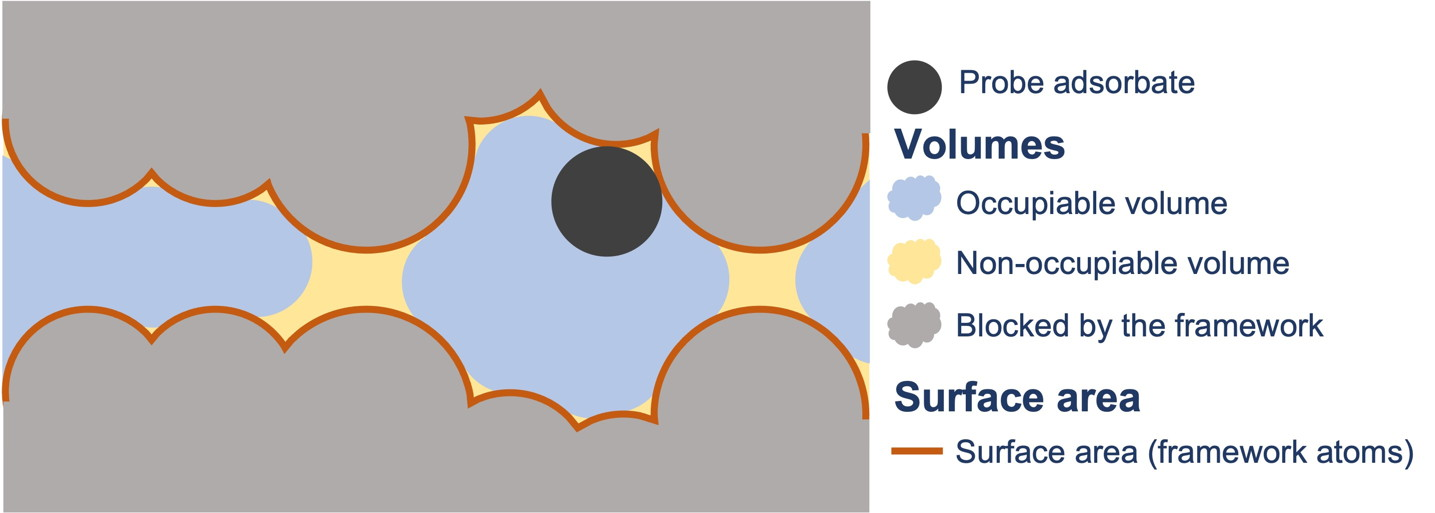
\includegraphics[width=0.7\textwidth]{figures/1-screening/Pore_descriptors.jpg}
  \caption{Illustration of the pore surface area and volume in a nanoporous material. As illustrated, there are different definitions of the pore volume: we can either consider the whole volume of the pores or the volume occupiable by a given probe. The surface area also changes depending on the definition. Studies have shown that occupiable volume has a better accordance with experimental data.\cite{vol_Ongari2017}}\label{fgr:pores}
\end{figure}

%Definitions of surface area, porosity etc. Values depend on the method to extract them. A word on computational characterization (will be developed later)
The cavities of the nanoporous material lay out an incredibly large adsorbable surface area, which is extremely useful in increasing the number of molecules in a given volume or mass of material, several thousands of square meters can be found in a gram of some nanoporous materials.\cite{Farha_2012} The higher the surface area, the more molecules can be adsorbed for storage, separation or reaction purposes; it is therefore crucial to measure this surface area using experimental and computational methods. The most extensively used method to experimentally measure surface areas from adsorption isotherms is based on the Brunauer–Emmett–Teller (BET) theory.\cite{Detsi_2011} Most BET areas are calculated on \ce{N2} isotherm at its boiling temperature (\SI{77}{\kelvin}); although different probe adsorbates can be considered, they are not standard.\cite{Tian_2017} However, the definition of the surface area depends highly on the condition of measurement but also on the fitting methodology; a dozen isotherms were given to 61 labs for BET area calculation, and the statistical experiment yielded to a high level of disparities in the calculation.\cite{Osterrieth_2022} 

Beyond the experimental techniques, some software like Zeo++ or PoreBlazer focus on computing pore size distributions, surface areas and void fractions using well-defined structure files.\cite{Zeo++,PoreBlazer} The definition of these values also depends on the probe size chosen to model a given adsorbate, the size of the framework atoms and the quality of the input structure. The computational values do not rely on adsorption models or on isotherm data as in the BET area, they are now relying on more comprehensive structural data. As illustrated on the figure\ref{fgr:pores}, they, however, very much rely on a well-designed definition of the volume, the surface and the pore size we want to evaluate. Moreover, these values also highly depend on the radii of the framework atoms and the adsorbate we consider.\cite{Hung_2021}. In this thesis, we will rely on these computational methods to define these geometrical descriptors of nanoporous materials.

\subsubsection{Classes of nanoporous Materials}

\begin{figure}[ht]
  \centering
  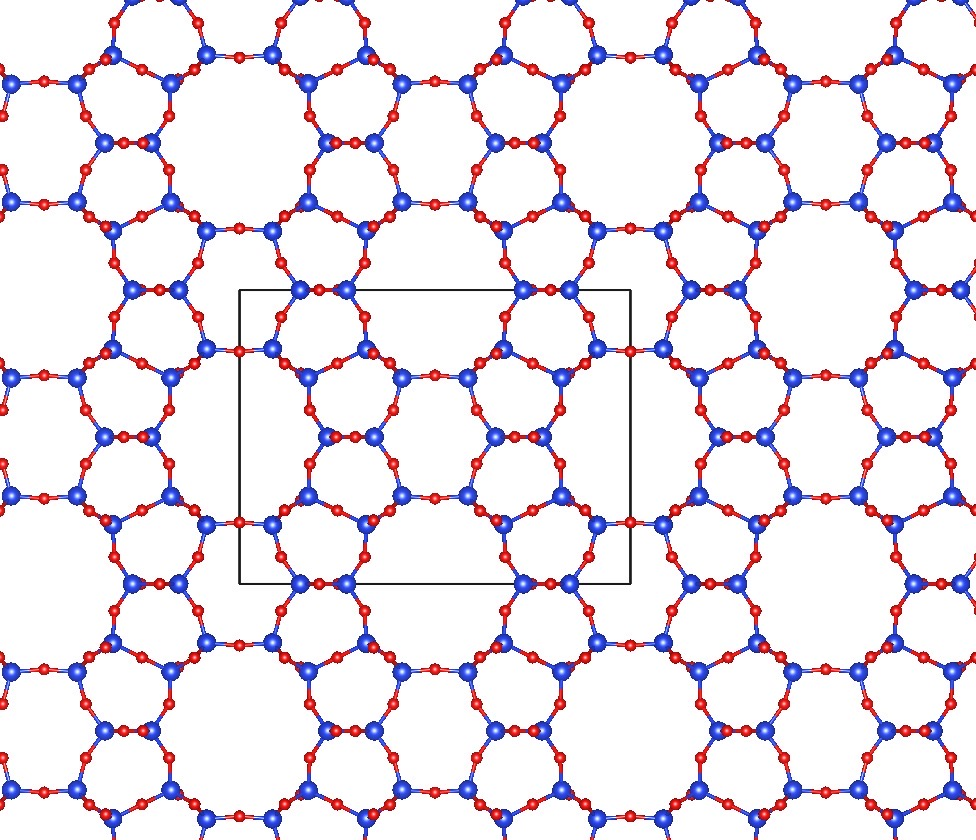
\includegraphics[height=0.23\textwidth]{figures/1-screening/FER.jpg}
  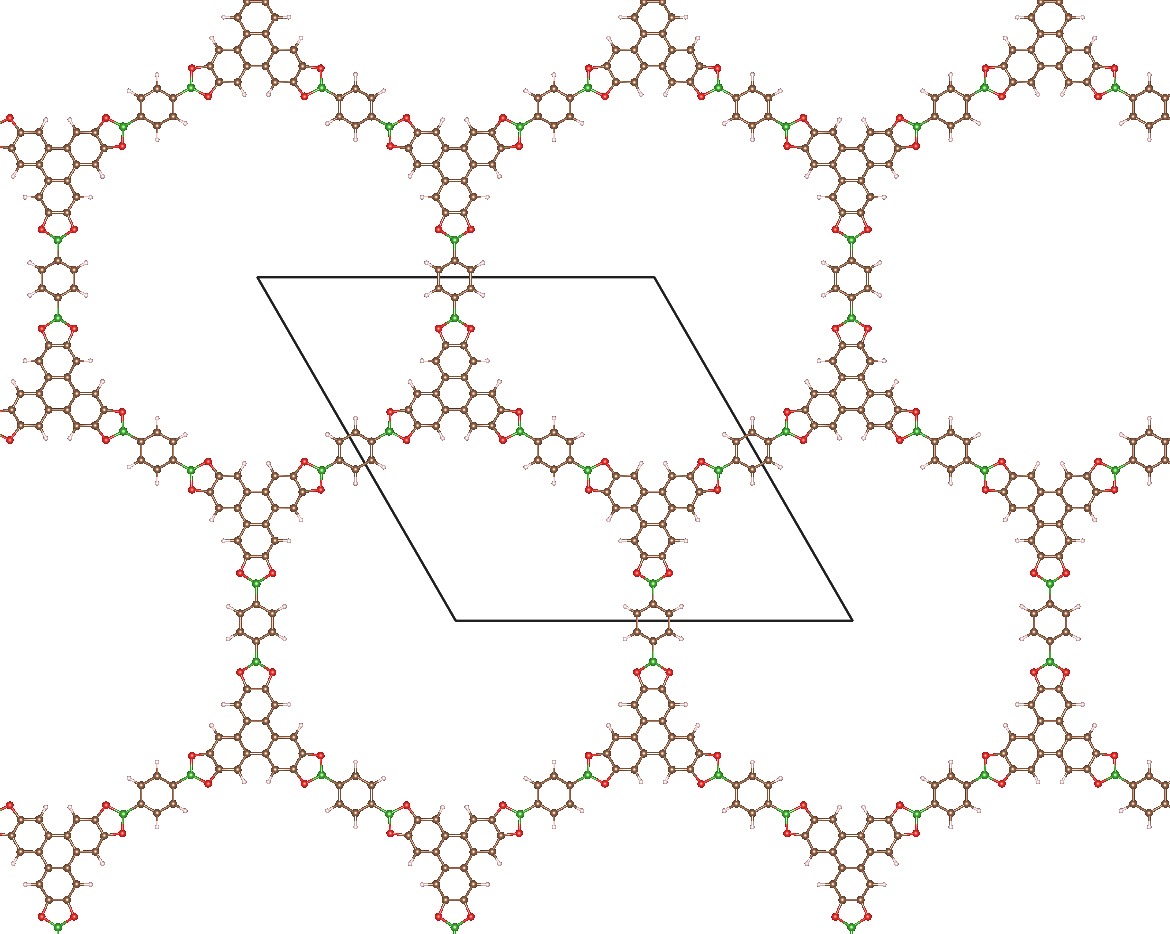
\includegraphics[height=0.23\textwidth]{figures/1-screening/COF-5.jpg}
  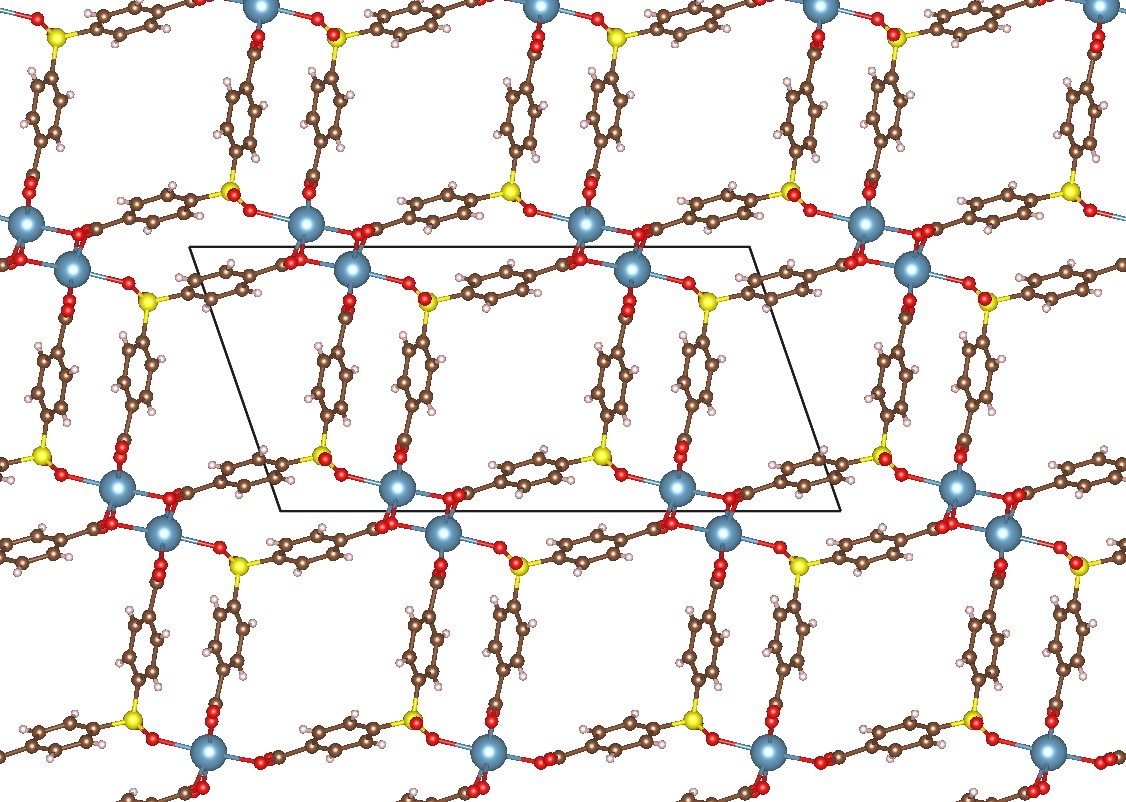
\includegraphics[height=0.23\textwidth]{figures/1-screening/SBMOF-1.jpg}
  \caption{Illustration of a zeolite FER\cite{FER}, a COF\cite{Cote_2005} and a MOF\cite{KAXQIL}. Color code: brown for C, white for H, red for O, blue for Si, cyan for Ca, yellow for S and green for B.}
\end{figure}

%Material classification crystalline / amorphous
Nanoporous materials can have different degrees of crystallinity from perfectly crystalline to completely amorphous. Most of the computational work is focused on crystalline structures, since the atoms are well described within a periodic framework, which enables faster simulations. The presence of defects is also usually neglected, which could explain some discrepancies between simulations and experiments. And amorphous materials are described by thousands of atomic positions in order to grasp their intrinsic non-periodicity.\cite{Thyagarajan_2020} Activated carbons, a famous class of amorphous material, are extensively used in the industry for gas purification, but cannot be rationally studied to characterize their adsorption properties. One can distinguish roughly three main classes of crystalline nanoporous materials: the inorganic materials like zeolites (aluminosilicates or aluminophosphates), the organic materials like the porous polymer networks (PPNs) or the covalent organic frameworks (COFs) and the metal--organic frameworks (MOFs).

Zeolites are naturally occurring nanoporous aluminosilicate materials that are commonly synthesized to be used in the industry as a commercial adsorbent and heterogeneous catalyst.\cite{Ozin_1989,Ma_2000} It is considered as one of the most mature nanoporous material technology at our disposal. This class of material also leaves a wide room for innovation since different Al/Si ratios of a same zeolite type pan out a wide range of structures. Furthermore, zeolite materials inspired the synthesis of zeolitic frameworks harboring different atoms such as the aluminophosphates or the zeolitic imidazolate frameworks.\cite{Wang_2012,Chen_2014_zeo} 

Porous polymer networks (PPNs) are porous materials based on the already very developed polymer material technology.\cite{Lu_2010,Wang_2020,Che_2020} However, one of the major drawback of this type of material is the formation of irreversible covalent bonds, which make the synthesis kinetically controlled leading to difficulties in crystallizing PPNs.\cite{Feng_2012} In order to create crystalline porous materials, Cote et al.\ figured out a way of using boron-based organic compounds to form reversible bounds, which formed thermodynamically stable materials COF-1 and COF-5.\cite{Cote_2005} This initiative was led by the group of Yaghi who was at the initiative of another very promising and well-known class of materials. A decade earlier,  they pioneered a hydrothermal synthesis of a metal--organic framework presenting broad rectangular channels.\cite{Yaghi_1995} 

Metal--organic frameworks (MOFs) are a class of nanoporous materials formed by metallic centers connected with organic linkers to form a stable crystalline solid. Even if the first synthesis of such a material was done since the early 90s,\cite{Abrahams_1991} and brought about a sparking interest in the scientific community a couple of decades later.\cite{Kuppler_2009,Furukawa_2013} Because plenty of combinations of linkers and metals are imaginable, an infinite amount of MOFs could theoretically be designed. Their structure can be tuned to our needs to enhance their performance in the targeted application.\cite{Ejsmont_2021} This diversity of nanoporous materials offer a wide range of potential candidates that could be evaluated for any targeted applications. 


\subsection{Computational Databases}

All the previously described materials have been either synthesized and resolved using X-ray crystallography or computationally constructed. By combining almost all possible nanoporous materials, almost a million structures have been considered for separation or storage applications.\cite{Simon_2015,Simon_2015_EES,Thornton_2017} This extended database can be broken down into the synthesized materials and hypothetical ones for all the above-mentioned classes of material.

%experimental
The International Zeolite Association (IZA) gave a standardized set of 244 zeolites (in their idealized all-silica form) that can be used for screening purposes. To generate a dataset of structures, existing experimental databases like the Cambridge Structural Database can be exploited. However, the raw structures determined experimentally by X-ray cannot be used directly as is. To obtain a computation-ready dataset, Chung et al.\ used algorithmic cleaning procedures to build the publicly available Computation-Ready Experimental MOF (CoRE MOF) database.\cite{Chung_2014, Chung_2019} CoRE MOF 2019 contains about 14,000 MOF structures, which is the biggest experimental database. Similar approach applied to organic frameworks led to the construction of a set of 187 COFs with disorder-free and solvent-free structures.\cite{Tong_2017,Ongari_2019}

%hypothetical
These experiment-based databases can already be used in computational screenings to retrieve valuable information, but unknown structures that are yet to be discovered are not represented. To overcome the limits and biases of experimental synthesis, artificial ways of generating nanoporous material datasets can be used, which proved to be extremely efficient. The first \emph{in silico} generated database of about 130,000 MOFs used a recursion-based assembly (or Tinkertoy-like) algorithm to combine 102 building blocks.\cite{Wilmer_2012} Martin and Haranczyk then proposed a topology-specific structure assembly algorithm that leverages the topological information of the structures.\cite{Martin_2014} Inspired by this algorithm, topology-based databases emerged a few years later with the set of 13,000 MOF structures generated using the Topologically Based Crystal Constructor (ToBaCCo) algorithm developed by Colon, G{\'{o}}mez-Gualdr{\'{o}}n and Snurr.\cite{Colon_2017} Later, Boyd and Woo proposed another topology-based algorithm using a graph theoretical approach and generated a 300,000-structure database (BW-DB) based on 46 different network topologies.\cite{Boyd_2016} Similar approaches are used for other classes of materials, Deem and co-workers proposed a dataset of nearly 2.6 million hypothetical zeolite structures.\cite{Earl_2006,Deem_2009,Pophale_2011} However, one could wonder if these hypothetical structures are synthesizable and can remain stable under operational conditions (e.g.\ thermal, mechanical, radioactive constraints). To discuss their synthetic likelihood, Anderson and G{\'{o}}mez-Gualdr{\'{o}}n computed the free energies of 8,500 hypothetical structures and compared them to experimentally observed MOF structures.\cite{Anderson_2020} Later, Nandy et al.\ performed a meta-analysis of thousands of articles associated to the CoRE MOF 2019 database to extract their experimental solvent-removal stability and thermal decomposition temperature.\cite{Nandy_2021} These data are then leveraged in the training of multiple ML models to predict stability properties. These predictions can be very useful to gauge the relative stability of each material and to only consider stable structures. Other types of materials have been explored, Turcani et al.\ published 60,000 organic cage structures and used machine learning to predict their stability based on the shape persistence metric.\cite{Turcani_2018}

The Materials Genome Initiative, a 100 million dollar effort from the White House that aims to ``discover, develop, and deploy new materials twice as fast'', led to the creation of the ``Materials Project'', a centralized database containing all the above-mentioned structures.\cite{kalil2011national,Matgenome,Jain_2013}
The fast development of this nanoporous materials genome motivated Boyd et al.\ to write a comprehensive review on all the initiatives on generating new data for computational analysis.\cite{Boyd_2017}

Yet, the sole increase in size of the databases is not enough. One needs to add diversity to have more general knowledge on the maximum performance and the explanatory features of such performance. Moreover, the diversity of structures ensure the quality of the predicted best materials for a given application. To qualitatively or quantitatively assess the diversity of a database, inventive methodologies have been developed. For instance, Martin, Smit and Haranczyk proposed a Voronoi hologram representation as a way of measuring similarities between structures to generate geometrically diverse subsets of a database.\cite{Martin_2011} Moosavi et al.\ made a comparative study of the diversity of three well-known databases CoRE MOF 2019,\cite{Chung_2019} BW-DB\cite{Boyd_2016} and ToBaCCo\cite{Gomez_Gualdron_2016, Colon_2017}  using geometrical and chemical descriptors to design a theoretical strategy for generating the most diverse set of materials.\cite{Moosavi_2020} Another approach consists in searching for similarities instead of differences in the materials by studying topological patterns in the data.\cite{Lee_2017} These investigations on the data structures give a solid ground to develop novel materials by objectively defining similarity, diversity and novelty. From the analysis gathered so far, one would need to radically change the approach by proposing materials with new chemistry, topology or mechanism (e.g.\ flexibility) in order to significantly improve the diversity of the current databases.


\subsection{Exploring the Chemical and Structural Space}


With the development of ever-increasing nanoporous material databases, computational chemists proposed more and more inventive methods to evaluate or screen thousands of structures. Other challenges arose, such as the design of more efficient methods than the brute force screening or the analysis of big data. Two research groups in Northwestern University led by R. Snurr and J. Hupp began to address those questions, they used a ``funnel-like'' approach to efficiently screen about 130,000 hypothetical MOF structures.\cite{Wilmer_2012} To do so, they performed a first screening involving fewer steps of simulation on the whole dataset, then they extracted a subset of top-performing structures to perform a second round with more simulation steps. This procedure is repeated until a few materials are selected by a final round of simulations with reasonable accuracy. Similar ``funnel-like'' procedures have then been used in other fields of applications as described in the Figure~\ref{fgr:screening}. This type of screening saves precious computation time by balancing the complexity of the calculation with the amount of data to be screened. The most demanding simulations or experiments are only applied to the few most promising structures. This method can rather efficiently identify top candidates, but it can't draw quantitative structure-property relationships (QSPR), beside facing scalability issues above a critical dataset size.

To overcome these new challenges, people are looking increasingly towards transferable models trained by a machine learning (ML) algorithm on a diverse and size-limited subsample. Ideally, such a model is transferable to potentially millions of structures and can provide valuable QSPR. For instance, Fernandez et al.\cite{Fernandez_2013} used multiple linear regression analysis, decision tree regression, and nonlinear support-vector machine models to extract QSPR and establish rules of designing well-performing MOFs for methane storage, while identifying promising structures. In this first work, they only used geometrical descriptors to describe methane storage,\cite{Fernandez_2013} but realizing the importance of chemical descriptors, they proposed the atomic property weighted radial distribution function as a powerful descriptor to predict \ce{CO2} uptakes.\cite{Fernandez_2013_rdf} More importantly, they proved that ML can be used as a pre-screening tool to avoid running time-costly simulations by correctly identifying around \SI{95}{\percent} of the top 1000 best performing materials. Recently, the same group used similar techniques to predict \ce{CO2} working capacity as well as \ce{CO2}/\ce{H2} selectivity in MOFs for pre-combustion carbon capture.\cite{Dureckova_2019}

\begin{figure*}[t]
    \centering
      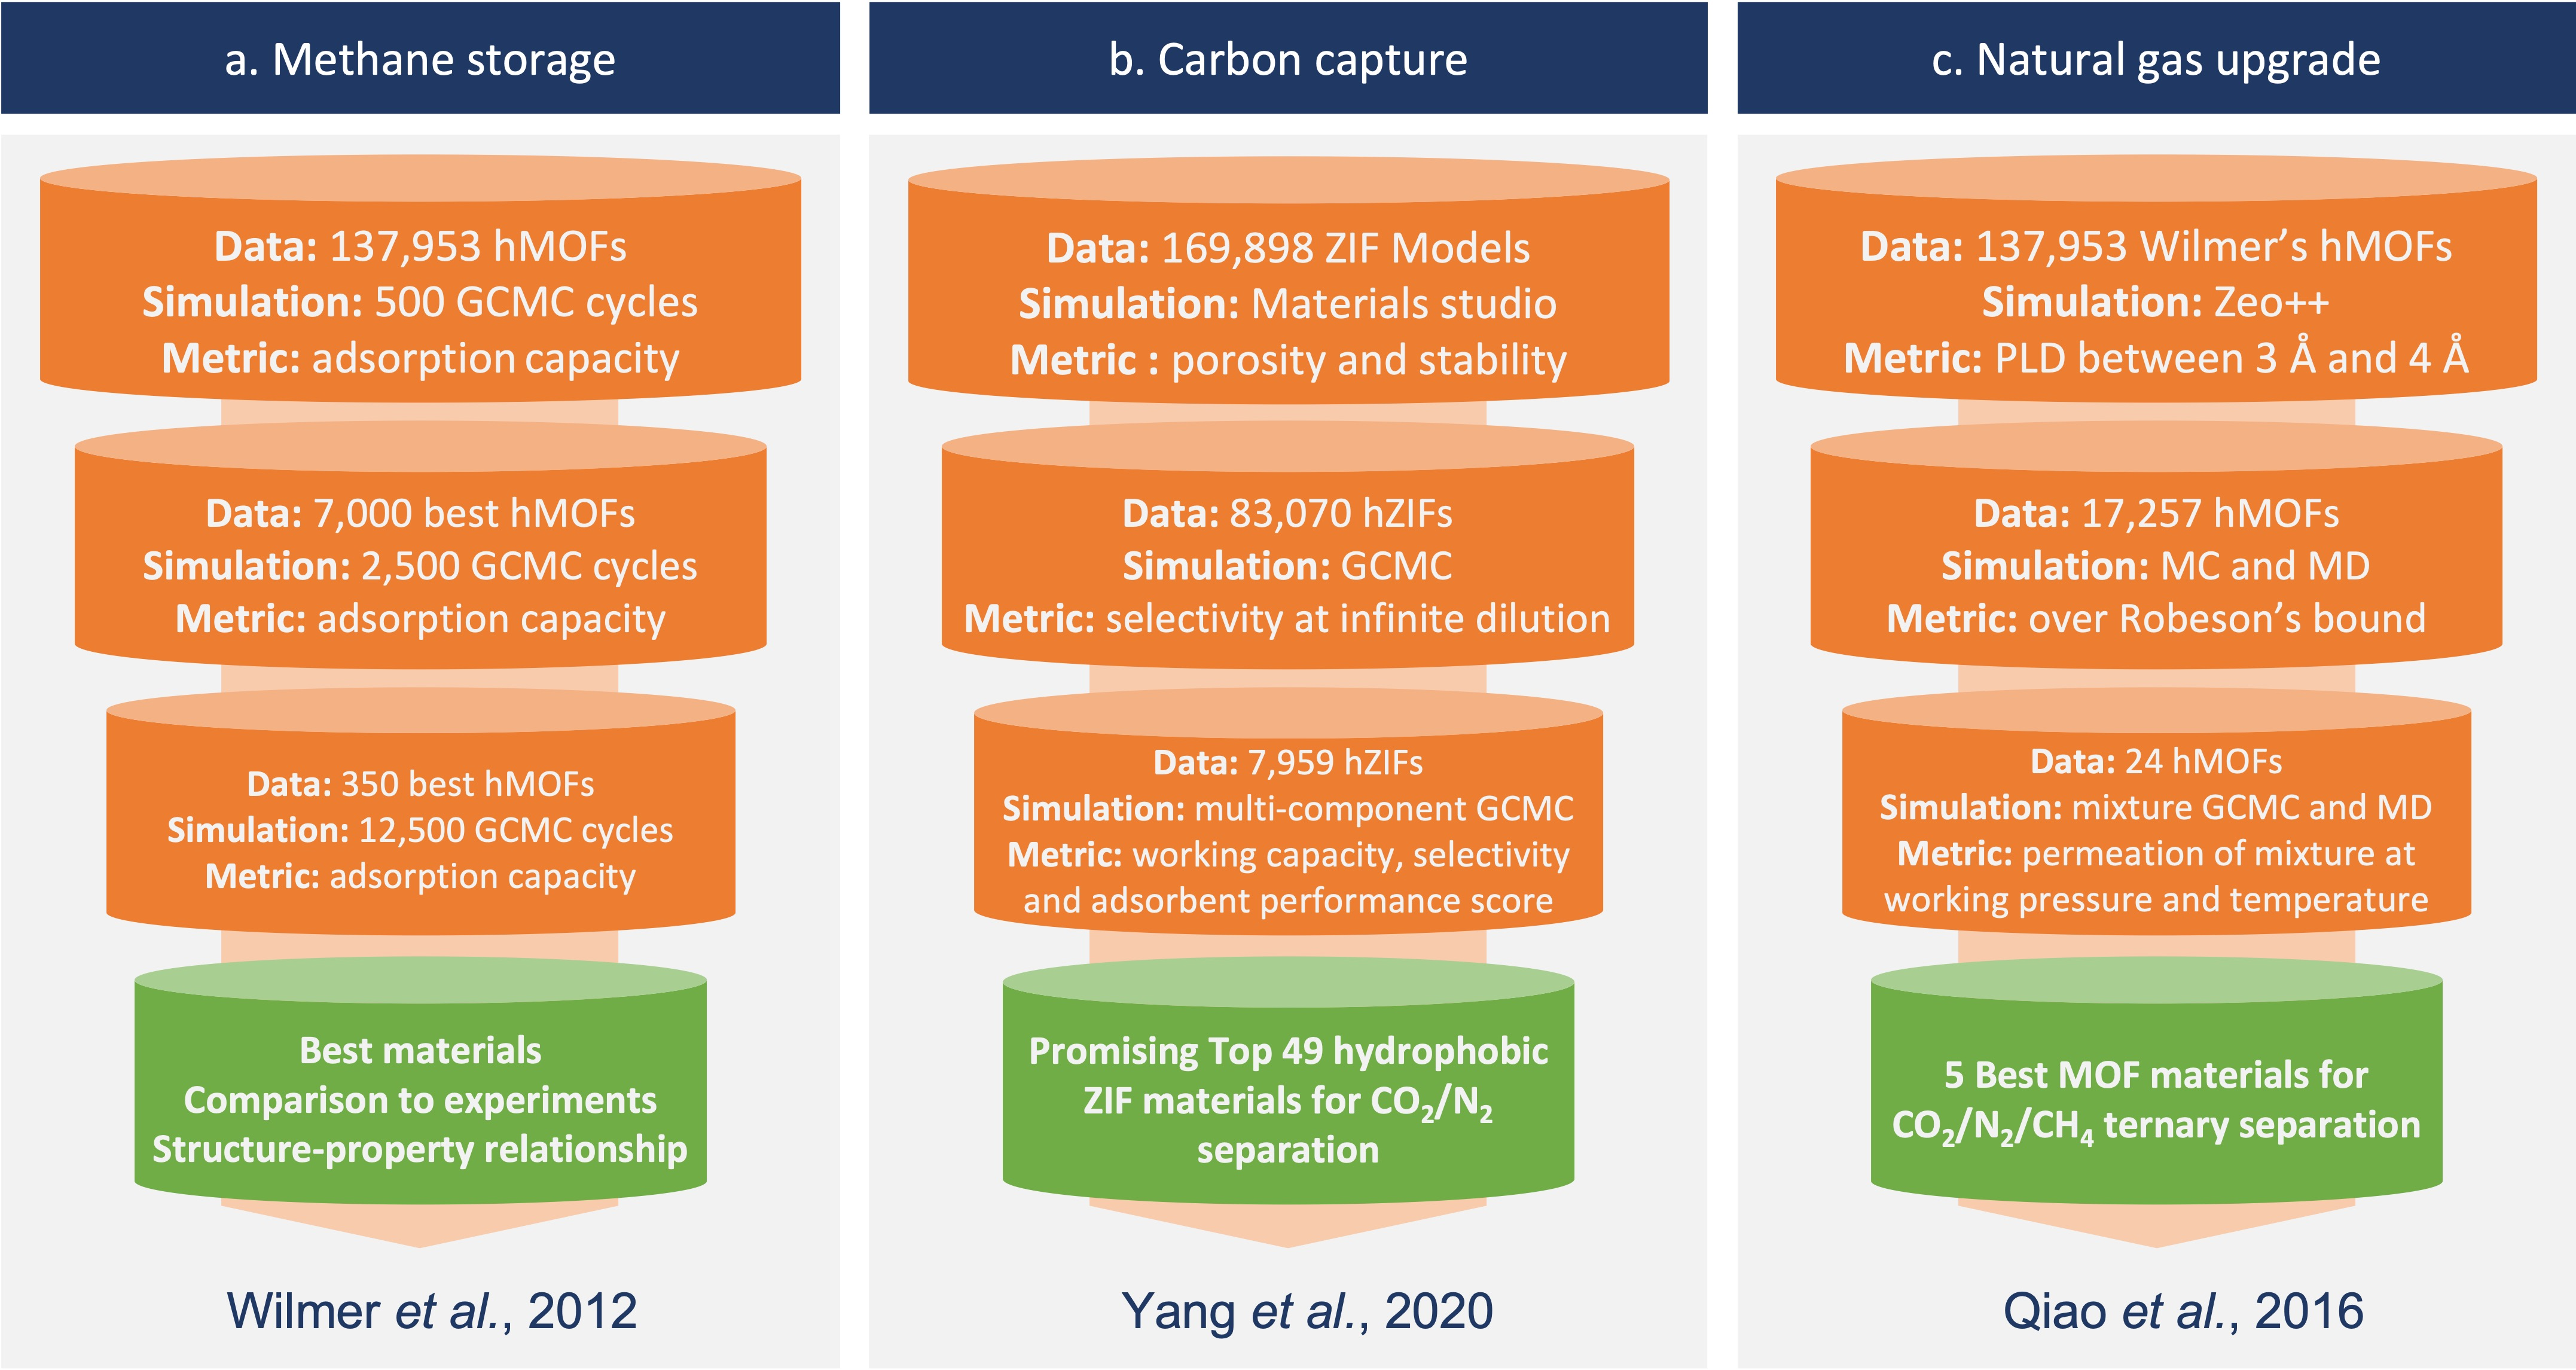
\includegraphics[width=0.98\textwidth]{figures/1-screening/Screening_procedures.jpg}
      \caption{Simplified representation of typical funnel-type screening procedures, exemplified on three different applications from the published literature. (a) Wilmer et al.\cite{Wilmer_2012} used a series of bi-component Grand Canonical Monte Carlo (GCMC) calculations at different levels of complexity to screen a large dataset of hypothetical MOFs for methane storage application. (b) Yang et al.\cite{Yang_2020} used simulations at infinite dilution to prescreen the dataset before using computationally demanding simulations and multiple metrics to find the most promising ZIFs for carbon capture. (c) In Qiao et al.\cite{Qiao_2016}, transport properties were screened along standard adsorption properties to find the best materials for the targeted \ce{CO2}/\ce{N2}/\ce{CH4} ternary separation; similarly, cheaper calculations at infinite dilution were carried out in a first step, before using more expensive calculations at working pressure and temperature.}\label{fgr:screening}
    \end{figure*}


\section{An overview of screening methodologies}


\subsection{Non-adsorption properties}

Due to their high internal surface area, adsorption applications were a natural outlet for nanoporous materials. However, these materials can be used in many other applications. This section is dedicated to the physical and chemical properties not directly related to the adsorption process inside nanoporous materials such as catalytic activity,\cite{Singh_2015, Greeley_2006, Back_2020}
mechanical properties,\cite{Chibani_2019, Gaillac_2020}
or thermal properties.\cite{Toher_2014, Sarikurt_2020, Ducamp_2021} These properties require a more refined description of the atomic interactions within the material. DFT simulations are usually performed to accurately retrieve these properties. However, the computational cost required is multiplied by several orders of magnitude compared to classical simulations. The size of the datasets screened is therefore much smaller (a few hundreds maximum), and the use of ML can potentially speed up the whole process. ML is based on lower-cost descriptors,\cite{Evans_2017, Ducamp_2022} or it can be used in ML potentials for molecular simulations\cite{Eckhoff_2019,Friederich_2021}.

\subsubsection{Catalytic Activity}

Beyond adsorption properties, screening procedures have been applied to chemical properties such as catalytic activities. Heterogeneous catalysis is generally performed using metallic nonporous structures, the use of nanoporous materials can increase dramatically the active surface area and the catalytic activity. Consequently, MOFs have been demonstrated to show catalytic properties for several chemical reactions. Just to cite a few, one can think of hydrogenation, hydrolysis, oxidation, among others explicitly covered by McCarver et al.\ in their review.\cite{McCarver_2021}
Considering the sheer number of possible materials, computational studies are potentially more effective than experimental ones. Therefore, computational screenings evolved in the last decade aiming at studying more sizable datasets.

Although the vast majority of computational screenings have been done on small series, there are a few systematic screenings of bigger datasets. The scarcity of the latter can be explained by the high level of computational cost required. Here, we show some examples of such attempts by focusing on the example of C--H bond activation for the conversion of alkanes into alcohols in the presence of nitrous oxide.

Inspired by enzymatic catalysis of the reaction of small alkanes with \ce{N2O} into alcohols, Vogiatzis et al.\ identified  seven iron-containing MOF structures out of 5,000 structures from the CoRE MOF database.\cite{Vogiatzis_2016} They found two descriptors that govern the catalytic activity: 1) the N--O dissociation energy of \ce{N2O} on the adsorption site and 2) the energy difference between two spin states of the intermediate.
Using a screening on these descriptors, three structures were identified as promising for further experimental studies. The best one has been computationally demonstrated to catalytically and selectively oxidize ethane to ethanol in presence of \ce{N2O}. Moreover, the authors found that defects played a major role in the observed catalytic activity.

\begin{figure}[ht]
\centering
  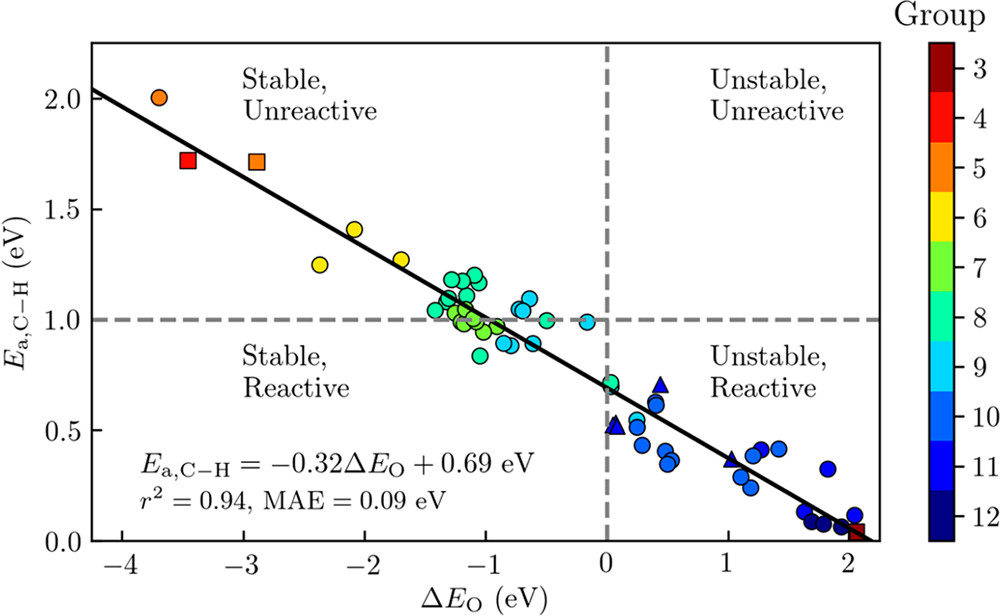
\includegraphics[width=0.8\linewidth]{figures/1-screening/Rosen_2019.jpeg}
  \caption{Analysis of a diverse set of experimentally derived metal--organic frameworks (MOFs) with accessible metal sites for the oxidative activation of methane. The graph shows the predicted barrier for the C--H bond activation of methane, E$_\text{a}$, as a function of the metal-oxo formation energy, $\Delta E_\text{O}$. For each material, the symbol color refers to the group number of the metal in the periodic table. The best-fit line has is plotted in black, and has a mean absolute error (MAE) of \SI{0.09}{\eV}. MOFs with E$_\text{a}<$ \SI{1}{\eV} are classified as being reactive towards C--H bond activation and MOFs with $\Delta E_\text{O}<0$ as having thermodynamically favored active sites when using \ce{O2} as the reference state. Reprinted with permission from Ref.~\citenum{Rosen_2019}. Copyright 2019 American Chemical Society.}
  \label{fgr:Rosen_2019}
\end{figure}

Later, Rosen et al.\ enlarged the scope of materials screened to other metals.\cite{Rosen_2019} From an 838 DFT-optimized MOFs subset of CoRE MOF 2014, the authors selected 168 MOFs that were likely to have open metal sites and pore-limiting diameters that allows the diffusion of the reactants. They then used a fully automated workflow to place the reactants in the adsorption site and relaxed the system using periodic DFT calculations. As shown in Figure \ref{fgr:Rosen_2019}, using the bond activation energy E$_\text{a,C--H}$ and the metal-oxo formation energy $\Delta E_\text{O}$ as key parameters, they classified the materials according to their relative stability and reactivity to find the best materials for the application. These energies were then analyzed using physicochemical descriptors such as the spin density on the oxygen and the metal--oxygen distance.

This type of brute force screening can be quickly cumbersome, as a result many researchers in the field are trying to find essential structure-activity relationships to accelerate future computational screenings.
Several descriptors have been developed for high-throughput screenings: Butler et al.\ used electron removal energies to explain photocatalytic behaviors of MOFs;\cite{Butler_2014} Rosen et al.\ showed that the energy required to form the metal oxide intermediate was a major descriptor of the thermal catalysis of alkane oxidation by \ce{N2O};\cite{Rosen_HTPDFT_2019} and Fumanal et al.\ show a screening protocol based on two energy-based descriptors to predict photocatalytic properties of MOFs.\cite{Fumanal_descriptor_2020} {Lately, Rosen et al.\ screened thousands of MOF structures to compare different DFT functionals and leveraged the data calculated to train machine learning models that can rapidly predict MOF band gaps.\cite{Rosen_2022_high} }

The development of ML methods are also critical in the field,\cite{Rosen_2021} but the lack of centralized database with high precision descriptors is a challenge for the future of these methods. The influence of defects, the different ways of modeling MOFs as periodic structures or clusters, the diversity of structures and the stability of such structures remain open problems. Yet, it does not threaten the major role of high-throughput screenings in the early design process of any nanoporous materials for catalysis. To conclude this brief overview, we point the readers to a more exhaustive presentation of the matter.\cite{Rosen_2022}

\subsubsection{Mechanical Properties}

In the past decade, there has been a growing interest in the systematic study of physical properties of various classes of materials, including inorganic materials and framework materials. Among these physical properties, mechanical properties have been a topic of particular interest, as they are crucial for many applications, and at the same time can be computed by relatively standard methodologies. In particular, is it possible to calculate linear elastic constants (the second-order elastic tensor) in the zero-Kelvin limit by strain/stress or strain/energy approaches, performing a series of DFT calculations of strained structures and calculating the elastic constants. From these constants, all other mechanical properties can be evaluated by tensorial analysis,\cite{Marmier_2010} including the bulk modulus, Young's modulus, shear modulus, Poisson's ratio, etc. This type of calculation can be coupled with any available quantum chemistry code,\cite{Golesorkhtabar_2013} and is even integrated in some packages, like CRYSTAL17.\cite{Dovesi_2018}

One of the first studies that investigated systematically the elastic properties of a family of materials was a 2013 study of all-silica zeolites,\cite{Coudert_2013} i.e., crystalline and porous Si\ce{O2} polymorphs. While this dealt with only 121 zeolitic frameworks out of 244 known structures, it showed that systematic studies at the DFT level were computationally tractable, and that they provided physical insight into the link between microscopic structure and macroscopic physical properties. This study demonstrated, among other things, that a few zeolites presented large negative linear compressibility (NLC), which could be linked to the wine-rack motif of their frameworks.

Outside the specific case of zeolites, other groups have applied DFT calculations of elastic constants in a high-throughput manner. de Jong et al.\ leveraged the structures of the Materials Project\cite{Matgenome, Jain_2013}, trying to chart the diversity of elastic properties across the whole space of inorganic crystalline compounds.\cite{deJong_2015} As shown in the Figure \ref{fgr:deJong2015}, they provided a database containing the full elastic information of 1,181 inorganic compounds initially, and has grown steadily since then, containing more almost 14,000 records to date.\cite{MaterialsProject} This dataset has been used in two different ways by researchers in the field.

Firstly, the exploration of the database of elastic properties by tensorial analysis has allowed studying quantitatively the occurrence of certain ``anomalous'' or rare mechanical behavior, including negative linear compressibility, very high anisotropy, or negative Poisson's ratio (also called \emph{auxeticity}). Indeed, such properties are considered rare and usually sought after --- the materials exhibiting these anomalous behaviors are mechanical metamaterials.\cite{Coudert_2019} In addition to their fundamental interest, such materials have applications in materials engineering: for example in energy dissipation (as shock absorbers and for bulletproofing), energy storage, as well as acoustics.\cite{Surjadi_2018} However, it was not possible until now to quantify exactly ``how rare'' they are. Chibani et al.\ showed through a systematic exploration of available mechanical properties of crystalline materials that general mechanical trends, which hold for isotropic (noncrystalline) materials at the macroscopic scale, also apply on average for crystals. Moreover, they could quantify the presence of materials with rare anomalous mechanical properties: {3\%} of the crystals were found to feature negative linear compressibility, and only {0.3\%} to exhibit complete auxeticity (negative Poisson's ratio in all directions of space).

\begin{figure}[ht]
\centering
  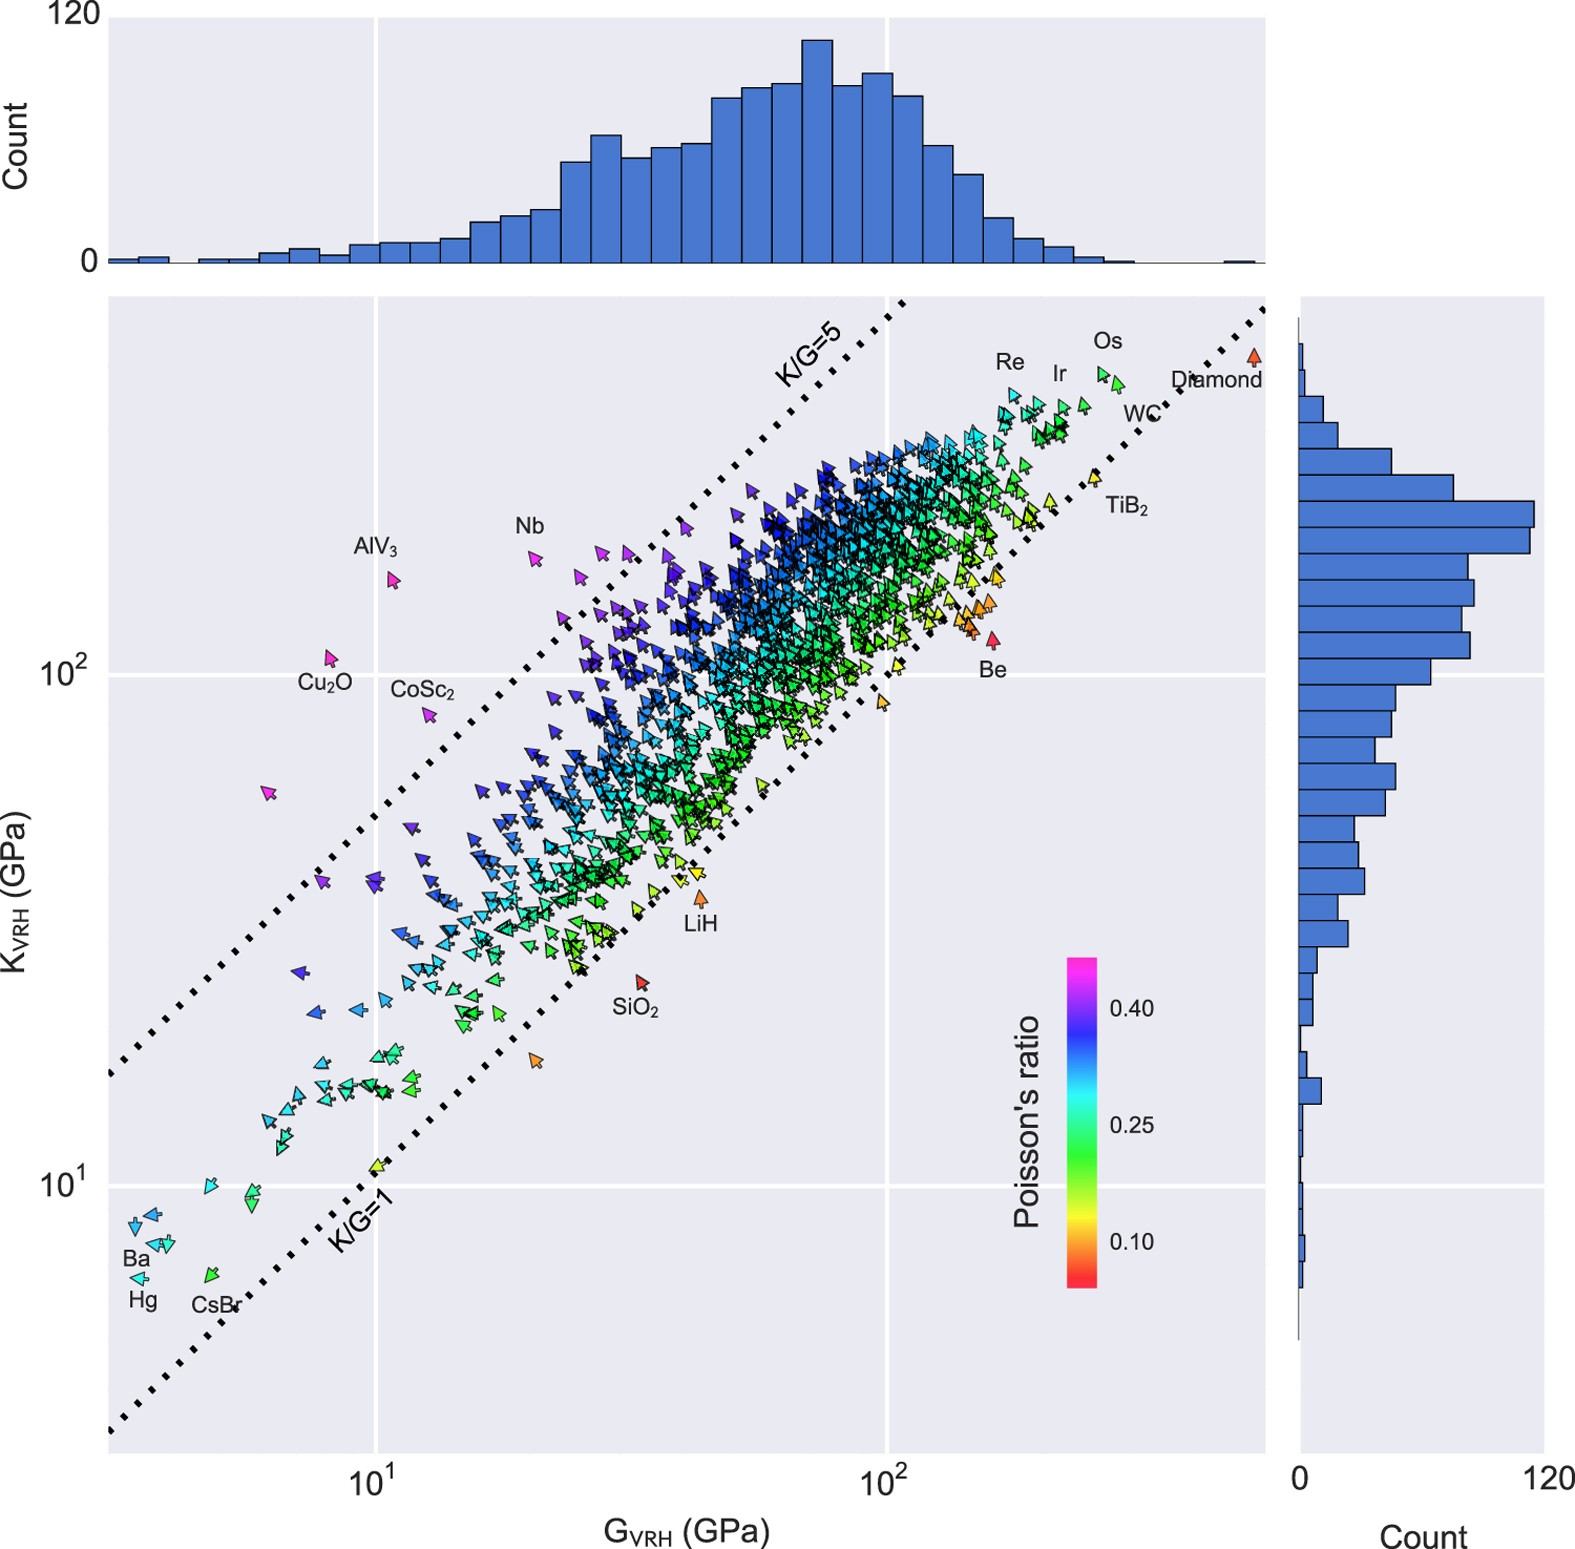
\includegraphics[width=0.8\linewidth]{figures/1-screening/deJong2015.jpeg}
  \caption{Statistical analysis of the calculated volume per atom, Poisson's ratio, bulk modulus {$\mathrm{K_{VRH}}$} and shear modulus {$\mathrm{G_{VRH}}$ of} 1,181 compounds in the Materials Project database. In the vector field-plot, arrows pointing at 12 o'clock correspond to minimum volume-per-atom and move anti-clockwise in the direction of maximum volume-per-atom, which is located at 6 o'clock. Reprinted from Ref.~\citenum{deJong_2015} under CC-BY license. Copyright 2015 de Jong \emph{et al}.}
  \label{fgr:deJong2015}
\end{figure}

Secondly, the datasets of mechanical properties were used as a basis to accelerate the discovery of novel materials with targeted behavior. Dagdelen et al.\ used search algorithms to identify 38 candidate materials exhibiting features correlating with auxetic behavior, from more than 67,000 materials in the Materials Project database.\cite{Dagdelen_2017} Performing DFT calculations on these 38 structures, they could identify 7 new auxetic compounds. In a more complex setup, Gaillac et al.~\cite{Gaillac_2020} have used a multiscale modeling strategy for the fast exploration and identification of novel auxetic materials. They combined classical force fields MD simulations with DFT calculations on candidate materials, and then used this reference DFT data to train an ML algorithm. They found that the accuracy of this multiscale method exceeds the current low-computational-cost approaches for screening. In a similar work, Moghadam et al.\ used molecular simulation to train an artificial neural network (ANN) for the prediction of the bulk modulus of metal--organic frameworks.\cite{Moghadam_2019} This shows the potential of such methodologies to treat very different (chemically as well as structurally) classes of materials.

\subsubsection{Thermal Properties}

While mechanical properties (in the elastic regime) have been by far the most studied physical property in nanoporous materials, others have also been occasionally screened. We can cite, in particular, the systematic study of piezoelectric tensors by de Jong et al., on almost a thousand crystalline compounds, by first-principle calculations based on density functional perturbation theory.\cite{deJong2015_piezo} We can also cite efforts to calculate thermal properties in a high-throughput setup, using the quasi-harmonic approximation (QHA).\cite{Togo_2010} This method requires the calculation of each structure's phonon modes at various volumes, and can be coupled to any electronic structure program.\cite{Togo_2015} It is, however, quite computationally intensive, and sensitive to the parameters of the QHA methodology (range of volume, range of temperature, precision of the frequency calculation, etc.). Therefore, it has been limited so far to modest numbers of structures: a dataset of 75 inorganic structures by Toher et al.,\cite{Toher_2014} and more recently a dataset of 134 pure Si\ce{O2} zeolites by Ducamp et al.\cite{Ducamp_2021} Very recent work in our group on the prediction of thermal properties through machine learning based on structural features alone indicates that thermal behavior is more difficult than mechanical behavior to predict, and might require the use of a wider set of structural descriptors or more advanced ML models.\cite{Ducamp_2022}


\subsection{Transport Adsorption Properties}

In the previous section, the thermodynamic properties only described the state of equilibrium of the adsorption process. But sometimes the transient state can last long before reaching the equilibrium, which makes the process more time-consuming. Thus, the transport properties complete the thermodynamic description of the adsorption process inside a nanoporous material. For example, a low diffusion rate would mean for storage applications more time and energy needed to fill-up the tanks, or for separation applications a less selective process than expected. In more extreme cases of molecular sieves for fluid separation, the transport properties become predominant to assess the performance. One can leverage the difference of the molecules' diffusion coefficients to selectively filter gas mixtures through a nanoporous membrane.\cite{Miandoab_2021} Here, the main subject becomes the transient state and not the equilibrium. This section is thus dedicated to the kinetics of the adsorption process to better model the time required to reach the equilibrium or to study out-of-equilibrium processes such as molecular sieving by nanoporous membranes.

\subsubsection{Kinetic Properties}

In most computational screenings, the diffusion coefficient considered is the self-diffusion coefficient that describes an infinite-dilution case. Other multi-component diffusion coefficients could be considered, but for simplicity and clarity they won't be mentioned in this review. The calculation of the self-diffusion coefficient gives a first estimation of the kinetics in a storage or a separation process in the limit of low adsorption loading.

There are two approaches to estimate the diffusion inside a porous material: the first one relies on molecular dynamics (MD) and the second one on transition state theories. In the first approach, one can analyze the mean squared displacement of the adsorbed molecule moving in the material. In the second, one identifies minimum energy path along the material to identify transition states (TS) to calculate diffusion energy barriers. The MD-based method requires fewer assumptions and is therefore more reliable than the TS-based method, but the latter is computationally more efficient in the case of low diffusion rate (diffusivity lower than 10$^{-11}$~\si{\square\meter\per\second}).

State-of-the-art MD simulations could calculate rather accurate diffusion coefficients, but the computational cost scales quickly with the number of structures. To use this method on a large dataset without spending too much computation time, Watanabe and Sholl prescreened the pore sizes of 1,163 MOFs to select only the structures within a certain range of PLD (pore limiting diameters).\cite{Watanabe_2012} A restricted list of 359 MOFs was then used to carry out MD simulations to calculate diffusion coefficients. The results of this final screening are then used to extract the most promising structures for further experimental or computational investigation. Similarly, Qiao et al.\ used a multistage screening to find the best membrane material within about 130,000 hypothetical MOFs for a \ce{CO2}/\ce{N2}/\ce{CH4} separation.\cite{Qiao_2016} They started to select materials based on pore geometry analysis; then they calculated Henry's coefficient and diffusion coefficients at infinite dilution; finally, they compared the binary permselectivities to extract 24 promising MOFs for ternary adsorption and diffusion calculation at the desired pressure and temperature conditions.

Another approach replaces MD simulations with more computationally efficient TS-based methods to determine diffusion coefficients.
Haldoupis et al.\ developed an algorithm to identify diffusion paths by exploiting an energy grid with a clustering algorithm. The diffusion paths are then analyzed to identify the pores and the channels, and to calculate key geometric (PLD, the largest cavity diameter) and energetic (Henry's constant, diffusion activation energy) features.\cite{Haldoupis_2010}
As illustrated in Figure \ref{fgr:Haldoupis_2010}, they found a clear dependence of the diffusion energy barrier to the PLD. As one of the first TS-based screenings, it is still subject to many development perspectives. For instance, the approach is limited to spherical adsorbates and rigid frameworks. Moreover, the diffusion coefficients are approximated using a simplistic hopping model for a qualitative analysis. This method is highly efficient, but the accumulation of approximations makes a quantitative systematic analysis of diffusion coefficients out of reach.

\begin{figure}[ht]
\centering
  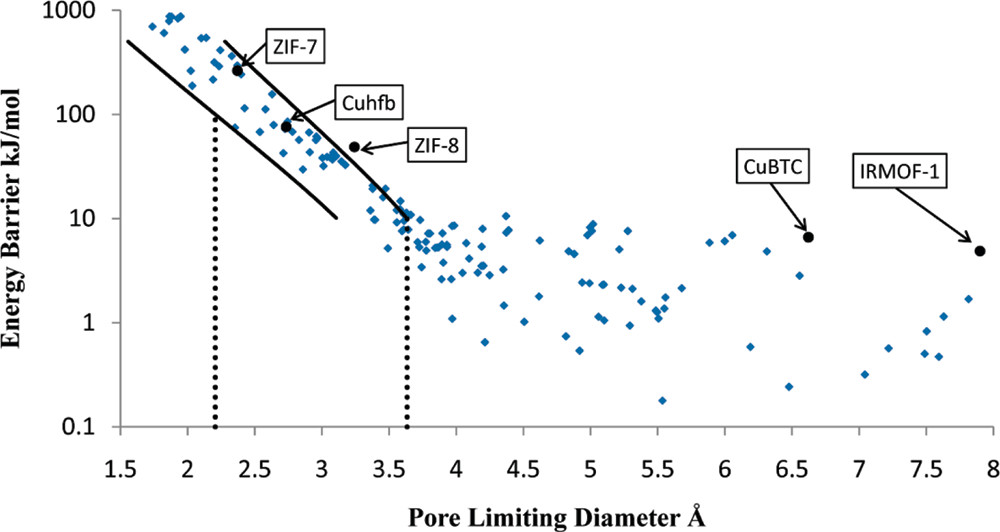
\includegraphics[width=0.7\linewidth]{figures/1-screening/Haldoupis_2010.jpeg}
  \caption{Calculated energy barrier for the diffusion of \ce{CH4} in 216 metal--organic frameworks (MOFs), shown as a function of the pore-limiting diameter. The solid lines represent statistical upper and lower bounds on the energy barrier, in a transition state theory approach. Reprinted with permission from Ref.~\citenum{Haldoupis_2010}. Copyright 2010 American Chemical Society.}
  \label{fgr:Haldoupis_2010}
\end{figure}

Later, Kim et al.\ introduced a flood fill algorithm to obtain all the points within a given energy.\cite{Kim_2013} These points are then identified as channels or blocked regions. Along the channels, local minimums of energy are defined as lattice sites and transition states are defined perpendicular to the diffusion direction. A random walk is then computed along the lattice sites with hopping rates defined according to the activation energy. A diffusion coefficient is then calculated in each three directions of the space and an average diffusion coefficient is finally determined.
A comparison with the MD method on the IZA zeolite structures shows good agreement, but there are still some discrepancies explained by correlated hops in the case of rapid diffusion or by the presence of complicated channel profiles. Inspired by this work, Mace et al.\ developed a similar method that progressively fill the energy grid to detect transition states, hence removing the previous restriction to orthogonal cells only.\cite{Mace_2019} The diffusion coefficient is now computed using a kinetic Monte Carlo simulation allowing the adsorbate to jump freely in all directions instead of restricting it in a single dimension. This new method, called TuTraSt, handles very complex diffusion paths (like in the AEI zeolite). This new approach seems to be promising as it is in good agreement with MD simulations, while being 2-3 orders of magnitude faster. However, the time performance could improve tremendously by translating it from Matlab to C++ and by implementing parallelization procedures.

Very recently a massively parallel GPU-accelerated string method has been implemented and shared publicly to compute very efficiently diffusion coefficients {based on the transition state theory}.\cite{Zhou_2021} The recent developments in the prediction of diffusion coefficients in nanoporous materials point towards a promising future for the screening of transport properties applied to even larger databases. Going further, Bukowski et al.\ reviewed thoroughly diffusion in nanoporous solids as an attempt to connect theory to experiments.\cite{Bukowski_2021}

\subsubsection{Membrane Materials}

In separation application, the study of the transport properties can evaluate the feasibility of the thermodynamic equilibrium, crucial for any bed separation process. If this separation is not feasible, kinetic separation or partial molecular sieving are to be considered. Some notable examples are air separation in zeolites using pressure swing adsorption,\cite{ruthven1990air} \ce{N2}/\ce{O2} separation in carbon molecular sieves,\cite{Reid_1999} or \ce{N2} removal from natural gas.\cite{Wang_2019} In kinetic separation, the valuable metric is not the selectivity anymore, but the permselectivity, i.e.\ the product of the selectivity and the permeability (ratio of diffusion coefficients). Therefore, the screening of diffusion coefficients gives complementary information to the thermodynamic selectivity screenings. Here, we give some examples of such screening and the main descriptors that partially explain the computed figures of merit.

To give an overview on the potential of computational screenings to predict transport properties, we are now going to focus on the membrane separation applied to natural gas upgrading. The separation of \ce{CH4} from \ce{N2} and \ce{CO2} is a crucial step of this upgrading process.
In 2016, a large-scale high-throughput screening (see Figure \ref{fgr:screening} for the approach) of hypothetical MOF membranes for upgrading natural gas has been performed using MD simulations.\cite{Qiao_2016} Qiao et al.\ confirmed the existence of MOF materials beyond the upper bound for \ce{N2}/\ce{CH4} and \ce{CO2}/\ce{CH4} separations determined by Robeson on a large set of polymeric membranes.\cite{robeson1991correlation} This Robeson's upper bound is systematically crossed by MOF materials in computational screenings, see as an example the Figure \ref{fgr:Altintas_2018}. This can be explained by the fact that MOFs perform better than polymeric frameworks and the simulations at this level of theory. They also identified 24 MOFs suitable for the ternary \ce{CO2}/\ce{N2}/\ce{CH4} separation using a multistage screening described in the previous section.

Two years later, Qiao et al.\ used the same approach to study this ternary separation on a database of synthesized structures.\cite{Qiao_2018} Applying machine learning techniques to their data, they performed a QSPR analysis. Using a principal component analysis, they notably found that the permeability is higher when materials have high PLD and void fraction coupled with low density and percentage of pores within a characteristic range. The opposite was found to be true for high membrane selectivity for the \ce{CO2}/\ce{CH4} separation. Using decision tree algorithms, they gave objective procedures of selecting the best separation membranes based on some key descriptors. Finally, they studied in detail some top performing materials found by a support vector machine algorithm.

Altintas and Keskin later performed a screening on the same database for \ce{CO2}/\ce{CH4} membrane separation to identify the best performing materials and perform more computationally demanding simulations.\cite{Altintas_2018} {The simulations in rigid structures at infinite dilution show numerous structures above the Robeson's upper bound as shown in the figure \ref{fgr:Altintas_2018}, this crossing of the upper-bound can be explained by either a better performance of MOF membranes compared to the polymeric membranes used by Robeson, or an overestimation due to oversimplified assumptions (infinite dilution, rigidity). But when higher pressures and flexibility are considered, the selectivity values are dropping down closer to the upper boundary}, hence confirming the overestimation of the performance in screenings {based on rigid approximations at infinite dilution}. \revrem{But the best performing materials are still above the Robeson's upper bound and can therefore be used in mixed matrix membranes with polymeric membranes.} Budhathoki et al.\ developed a screening methodology for MOFs in mixed matrix membranes for carbon capture applications by estimating permeation values in these composite materials using a Maxwell model.\cite{Budhathoki_2019} The authors even proposed a pricing for each material compared to their relative performance. Similar studies have been carried out on different materials, Yan et al.\ showed the influence of decorating COFs with different chemical compounds on the membrane selectivity.\cite{Yan_2018}

\begin{figure}[ht]
\centering
  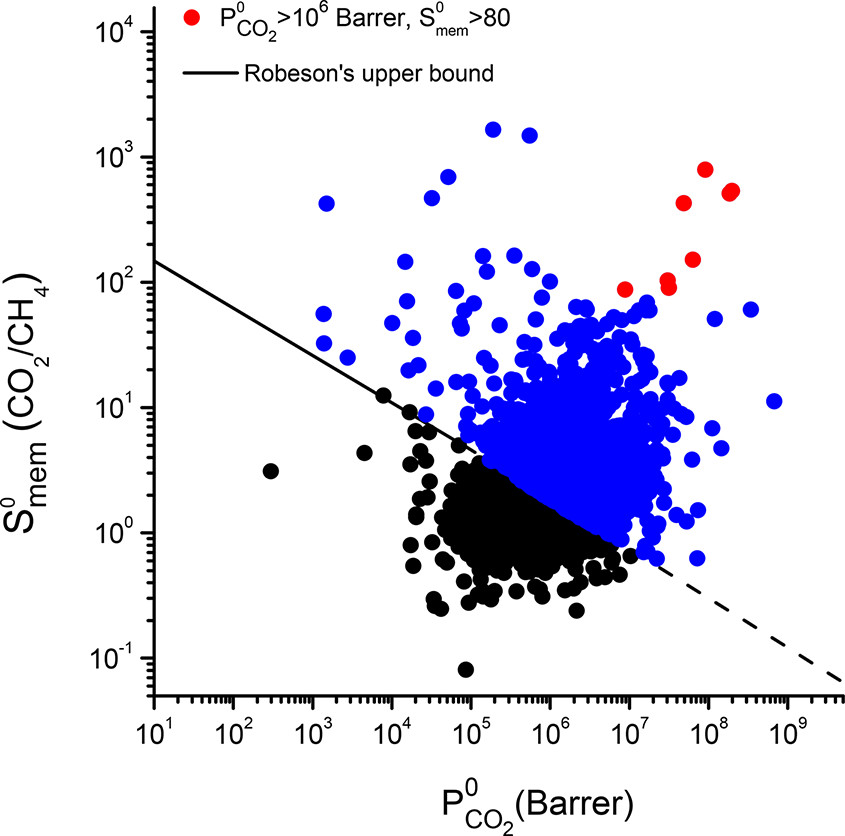
\includegraphics[width=0.5\linewidth]{figures/1-screening/Altintas_2018.jpeg}
  \caption{Selectivity and permeability of metal--organic framework (MOF) membranes for \ce{CO2}/\ce{CH4} separation computed at infinite dilution by combining Grand Canonical Monte Carlo and molecular dynamics simulations.\cite{Altintas_2018} The black solid line represents the Robeson's upper bound.\cite{robeson1991correlation, Robeson_2008} MOFs that can exceed the bound are shown in blue, and the 8 top-performing MOF membranes are shown with red symbols. Reprinted with permission from Ref.~\citenum{Altintas_2018}. Copyright 2018 American Chemical Society.}
  \label{fgr:Altintas_2018}
\end{figure}

The transport properties screening is based on the calculation of diffusion coefficients at infinite dilution and in rigid molecules. There are different methods to calculate them (mainly MD and TS-based methods). Flexibility and pressure dependence are very hard to incorporate directly in the screening procedures. Researchers usually consider these factors at the end of the screening on the most promising structures because of the computational complexity of the corresponding simulations. {To take account of} pressure dependence, {we need} an MD simulation of several adsorbates { that takes much more time than running single component simulations},\cite{Keskin_2007, Keskin_2009} which {makes it harder to include in a} high-throughput screening. Flexibility could be taken account by calculating snapshots and running multiple MD simulations, or by using flexible force fields, which means in both cases an increase in computational run-time. Some faster methods of quantitatively predicting the impact of flexibility on diffusion are being investigated in ZIFs and could give an interesting alternative to these expensive methodologies.\cite{Han_2020}

\subsection{Thermodynamic Adsorption Properties}

In its early development, computational screening was mainly used to predict thermodynamic properties in adsorption processes. Three main applications have been identified in the associated literature: gas storage (for energy or medical applications), gas separation (noble gas, hydrocarbons, carbon dioxide, etc.) and post-combustion \ce{CO2} capture. These applications are closely linked to urgent environmental and energy issues that are yet to be solved. Screening can guide the development of better performing materials by shedding light upon unknown structure-property relationship, probes possible theoretical limitations (unreachable targets) and identifies potential candidates that need to be experimentally tested.

\subsubsection{Gas storage}

One can leverage the high surface density of the nanoporous materials, especially the MOFs, to stock in very low-density gas. In the field of energy storage or transportation, natural gas (mainly methane) or hydrogen are considered plausible alternative fuels to replace conventional ones for transport. The US Department of Energy (US DOE) recently financed research programs and set targets for methane and hydrogen storage. Nanoporous materials could reduce energy, infrastructure and security cost due to the required compression and cooling. In this section, we are focusing on high-throughput screening for methane storage in nanoporous materials, before broadening the scope hydrogen and other perspectives.

One of the pioneering works in computational screening was published in 2012 by Wilmer et al.\cite{Wilmer_2012}. They performed a large-scale screening of 137,953 hypothetical MOF structures to estimate the methane storage capacity of each MOF at \SI{35}{\bar} and \SI{298}{\kelvin} based on the US DOE standards. Back then, the US DOE set a target methane capacity value of 180 vol{\footnotesize$^\mathrm{STP}$}vol$^{-1}$ (which has since been achieved by several materials reported in the literature). In their large-scale analysis, Wilmer et al.\ found over 300 hypothetical MOFs that meet the targeted requirements and the best one can store up to 267 vol{\footnotesize$^\mathrm{STP}$}vol$^{-1}$, surpassing the state-of-the-art of the time. From their large dataset, a preliminary structure-property relationship analysis revealed that void fraction values of approximately 0.8 and gravimetric surface areas in a range 2500-3000 m$^2$g$^{-1}$ resulted in the highest methane capacities. Optimal pore size is also shown to be around the size of one or two methane molecule(s). Maximization of gravimetric surface area was a common strategy in the MOF design for storage applications, but this study showed the existence of an optimal range of surface area values. Computational screenings can draw clear relationships between structural descriptors and performance. Later, a more quantitative relationship was drawn by Fernandez et al.\ using ML models as illustrated on Figure \ref{fgr:Fernandez_2013}. Beware not to over-interpret the relation given by the response surface, since the identified maxima do not always have a physical reality, especially where there is no training data in the area pointed by the red arrows. However, it highlights promising unexplored feature space and shows potential research directions.

\begin{figure}[ht]
\centering
  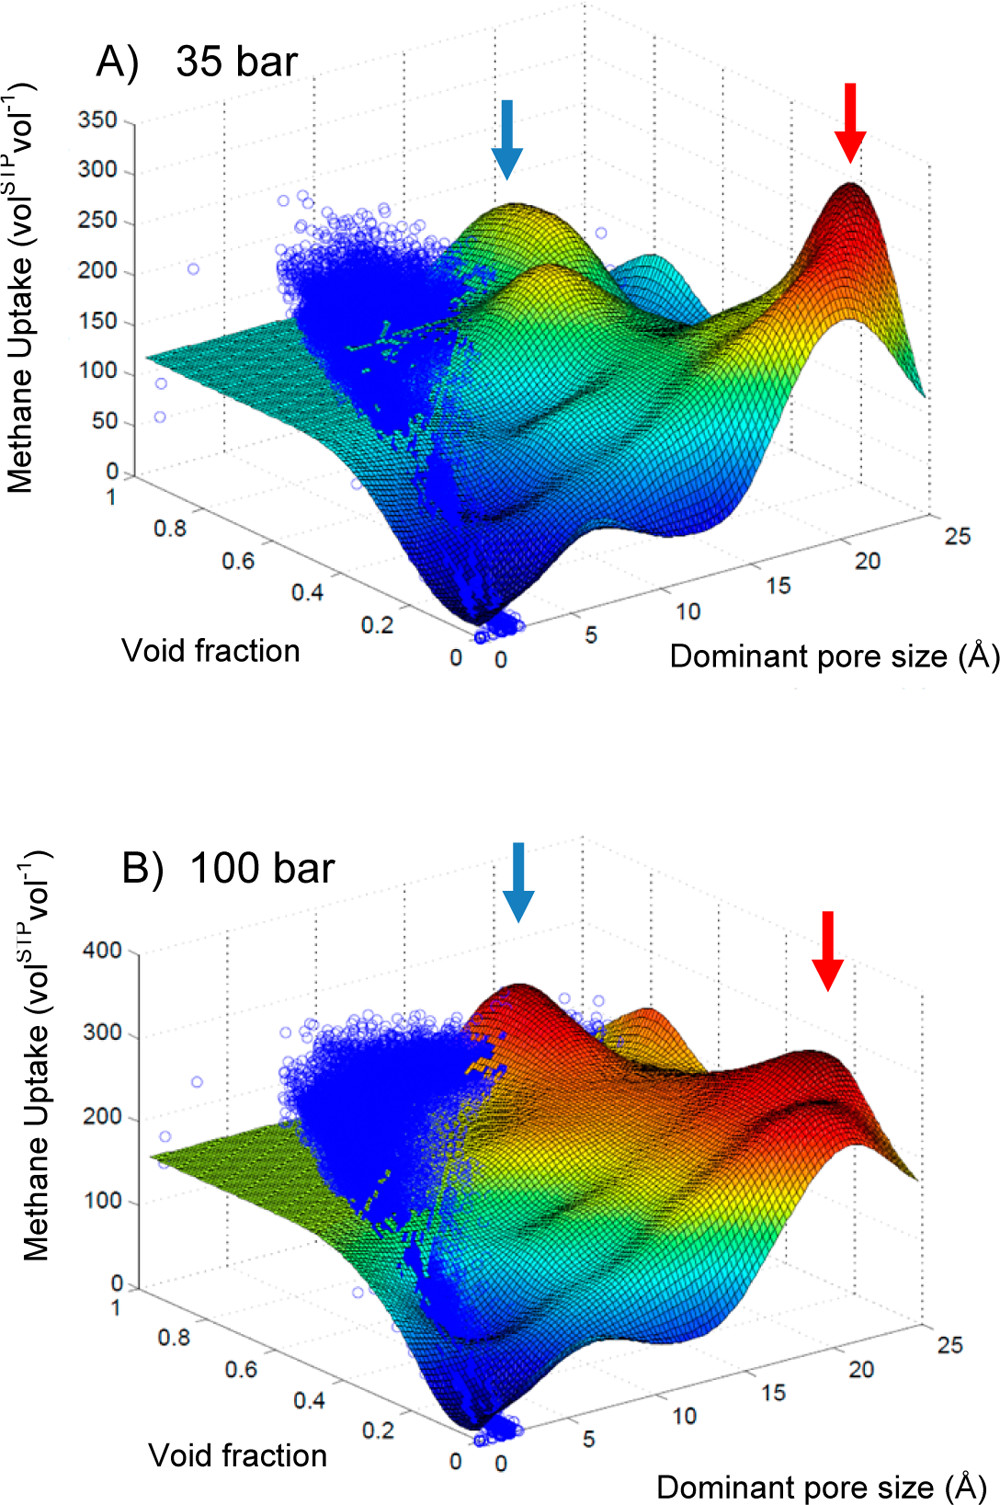
\includegraphics[width=0.5\linewidth]{figures/1-screening/Fernandez_2013_feature.jpeg}
  \caption{Two-dimensional response surfaces of the support vector machine (SVM) models trained by Fernandez et al.\ for methane storage at (A) 35~bar and (B) 100~bar using void fraction and dominant pore size. The blue dots represent the GCMC simulated uptake values. The color of the surface represents the methane storage value, from blue (the lowest values) to red (the highest values). Blue and red arrows indicate maxima on the response surface. Reprinted with permission from Ref.~\citenum{Fernandez_2013}. Copyright 2013 American Chemical Society.}
  \label{fgr:Fernandez_2013}
\end{figure}

Since then new materials above the target have been found and the US DOE decided to set a higher target of 315 vol{\footnotesize$^\mathrm{STP}$}vol$^{-1}$. Until now, this new target is not yet reached. This is why the recent developments have focused on assessing the feasibility of such a target by accelerating the screening methods so that more data can be screened, and by interpreting the QSPR models to extract important knowledge for the design of novel materials. For instance, G{\'{o}}mez-Gualdr{\'{o}}n et al.\ showed that even by artificially quadrupling the Lennard-Jones interaction factor $\epsilon$ and by increasing the delivery temperature by \SI{100}{\kelvin}, the newly set target is only reached by a handful of MOFs.\cite{Gomez_Gualdron_2014} This study suggests the impossibility to reach the DOE target using a preconceived (experimentally or theoretically) material to store methane. However, this theoretical limitation can be overcome by increasing the surface density of sites with high affinity with methane and by increasing the delivery temperature.

Later, a larger-scale screening on methane storage was carried out by Simon et al.\ on 650,000 experimental and hypothetical structures of zeolites, MOFs, and PPNs. This study confirmed that the classes of materials currently being investigated were unlikely to meet the new target. The authors suggested that it wasn't surprising since the target was based on economic arguments, while the screening is based on thermodynamic arguments.\cite{Simon_2015_EES} This example illustrates the power of large-scale screening to settle questions of physical feasibility (if simulations are accurate) and hence avoiding experimental efforts spent on impossible tasks.

More recently, a dataset containing trillions of hypothetical MOFs have been screened for methane storage.\cite{Lee_2021} Lee et al.\ developed a methodology using machine learning combined with genetic algorithm to perform the largest screening until now. In addition to confirming most of the results (theoretical limits and QSPR) found by previous screenings, 96 MOFs were found to outperform the current world record. This study shows the scaling potential of ML-assisted screenings in handling ``Big data''.

Similarly, computational high-throughput screenings have been applied to other storage applications such as hydrogen storage. Computational screenings showed that cryogenic storage of hydrogen can meet the DOE target of \SI{50}{\gram\per\liter}.\cite{Gomez_Gualdron_2016, Bobbitt_2016, Thornton_2017} Anderson et al.\ performed a large-scale screening based on neural networks to test out multiple pressure/temperature swing conditions to find that the maximal deliverable capacity cannot exceed \SI{62}{\gram\per\liter}.\cite{Anderson_2018} Compared to the density of liquid hydrogen (\SI{72}{\gram\per\liter}), this upper limit seems reasonable since the adsorbent material takes at least {10-20\%} of the tank. Here, we only showed some flagship results of the field. For a more detailed meta-analysis, Bobbitt and Snurr wrote a very complete review on computational high-throughput screening of MOFs for hydrogen storage.\cite{Bobbitt_2019}

\subsubsection{Xenon/krypton Separation}

As a representative example of what could be done in the field of gas separation, we are going to focus on Xe/Kr separation. Nanoporous materials can be used as a safer, cheaper and less energy-intensive option for this gas separation. However, experimental design of top-performing materials can be cumbersome. Computational screenings is an ideal tool to kick-start the development of this new technology by identifying rapidly the best candidates.

\subsubsection{Small-scale Screenings}

Metal--organic frameworks, and later other supramolecular porous materials like covalent organic frameworks (COFs), have been proposed for applications in separation of noble gases for a decade. With no aim of being exhaustive, we highlight some milestones in that area, both from experimental and computational point of view.

In 2012, Liu et al.\cite{Liu_2012} published an experimental study of two MOFs, HKUST-1 and Ni/DOBDC, for adsorption of Xe and Kr at ppm (part-per-million) levels in air. The target application was the removal of Xe and Kr from nuclear fuel reprocessing plants. The same group later proposed a two-column method for the separation of Kr and Xe from process off-gases\cite{Liu_2014}, based on MOF materials. At about the same time, Bae et al.\cite{Bae_2013} combined a computational Grand Canonical Monte Carlo (GCMC) study with experimental breakthrough measurements of the separation of a Xe/Kr mixture on MOF-505 and HKUST-1.

Parkes et al.\cite{Parkes_2013} studied sixteen different MOF materials for Kr, Ar, and \ce{N2} adsorption and separation, through GCMC simulations. They concluded on the potential of MOFs for separation, and a general correlation between the Henry's constant and the isosteric heat of adsorption for the three gases studied. A year later, in 2014, Chen et al.\cite{Chen_2014} demonstrated, again through a combined computational and experimental study, the potential of porous organic cages for selective binding of xenon over krypton.

Later experimental work expanded these early separation studies to different types of MOF materials. Xiong et al.\cite{Xiong_2015} studied a flexible zinc tetrazolate framework for xenon selective adsorption over krypton, argon and nitrogen. Thermodynamic analysis of the adsorption isotherms at various temperatures confirmed the occurrence of a ``breathing'' structural transition upon Xe uptake, contributing to a high working capacity for a pressure swing adsorption (PSA) cycle. Lee et al.\cite{Lee_2016} compared the selective adsorption properties for Xe/Kr mixtures on three highly studied MOFs, namely UiO-66(Zr), MIL-100(Fe) and MIL-101(Cr), and confirmed a high potential of UiO-66(Zr) for separations under dynamic flow conditions. These authors also assessed the hydrothermal and radioactive stability of the material, a test seldom performed in the existing literature, and found it to be good. In a further study,\cite{Lee_2018} they demonstrated that Xe/Kr selectivity could be further improved by ligand substitution.

In parallel, computational studies were published to provide insight at the microscopic level into the mechanisms behind good (and bad) separation properties. Wang et al.\cite{Wang_2014} studied 6 MOFs and COFs for adsorption of Xe and Xe/\ce{N2} separation, through GCMC simulations looking at the impact of pressure (and therefore pore filling) on selectivity. Anderson et al.\cite{Anderson_2017} combined GCMC and biased MD simulations to elucidate the nature of adsorption- and diffusion-based Kr/Xe separation mechanisms in four archetypal nanoporous materials: SAPO-34, ZIF-8, UiO-66, and IRMOF-1. These authors draw a couple of general conclusions, including the fact that diffusion selectivity for krypton dominates membrane separation selectivity, and large pore cages and stiff pore windows are desirable --- however the scope of these conclusions is inherently limited by the small number of materials actually studied.

In a different family of materials, Tong et al.\cite{Tong_2017} have surveyed the structure--property relationships of covalent organic frameworks (COFs) for noble gas separation, by GCMC simulations of 187 different materials for Kr/Ar, Xe/Kr and Rn/Xe separations. These authors included in their calculations some adsorption figures of merit (AFM), representative of the conditions of industrial vacuum (VSA) and pressure swing adsorption (PSA) processes.

One area that has been particularly explored is the tuning and improvement of separation properties through the presence and nature of coordinatively unsaturated sites (or open metal sites) in MOFs. In 2016, Vazhappilly et al.\cite{Vazhappilly_2016} used density functional theory (DFT) calculations of host--guest binding energies to probe the impact of the metal atoms in a specific framework (MOF-74) on Xe and Kr adsorption. Later, Zarabadi-Poor et al.\cite{ZarabadiPoor_2018} investigated --- again through computational methods --- a series of metal--BTC MOFs for recovering xenon from exhaled anesthetic gas, i.e., mixtures of \ce{CO2}, \ce{O2}, and \ce{N2}.

\subsubsection{Large-scale computational Screening}

In its early stage, computational screening has been used on a small series of nanoporous materials to generate specific knowledge on some subclasses of materials. These small-scale screenings combined with experiments helped faster identification of good performing candidates, but they failed to establish general rules of design or to explore the unknown. Larger-scale screenings overcame these limitations by trying to exhaustively cover the whole spectrum of nanoporous materials.

The first large-scale computational screening on Xe/Kr adsorption-based was performed by Sikora et al.\ based on the same approach previously developed for methane storage by their group at the Northwestern University.\cite{Sikora_2012} This study was based on the same {137,000} structures of hypothetical MOFs.\cite{Wilmer_2012} They calculated the Xe/Kr selectivity using Monte Carlo molecular simulations on the whole database by iteratively increasing the number of steps and selecting the best materials similar to the approach on Figure \ref{fgr:screening}. By analyzing the relationships between pore sizes and selectivity, they confirmed a hypothesis from a smaller scale study that the pores should be between the size of 1 to 2 xenon molecules.\cite{Ryan_2010} Tube-like channel was also found to favor better selectivity. Moreover, they found that top performing materials could have a selectivity around 500; but we can only conclude on the order of magnitude of the theoretical limitation of the Xe/Kr selectivity, considering the statistical uncertainty of the simulation.

Seizing the opportunity of a formidable expansion of the nanoporous materials database triggered by the Materials Genome Initiative, Simon et al.\ screened 670,000 experimental and hypothetical nanoporous material structures for Xe/Kr separation.\cite{Simon_2015} It is one of the largest-scale screening performed in this area. Inspired by the work of Fernandez and co-workers,\cite{Fernandez_2013} they used ML algorithms to train a model on a diverse subset of 15,000 structures. This method allowed them to run time-consuming molecular simulations only on this training set, before applying the ML model to predict the selectivity values on the larger set of structures. On top of analyzing the links between pore descriptors and selectivity, they rationalized it using theoretical pore models of spherical and cylindrical geometries to confirm the findings of Snurr and co-workers.\cite{Ryan_2010,Sikora_2012} By comparing the structural descriptors of good-performing and bad-performing structures, they concluded that geometrical descriptors wasn't enough to explain the performance (see Figure \ref{fgr:Simon2015}). The analysis of a few top candidates suggests that different chemical insights could explain their good performance. For SBMOF-1 or KAXQIL,\cite{KAXQIL} an experimental MOF, its higher performance was explained by the tube-like 1D channel with a very favorable binding site formed by carbon aromatic rings. This nanoporous material was later tested using breakthrough experiments and proved to be one of the most promising candidates.\cite{Banerjee_2016} This close collaboration between computation and experimentation is a testimony of the potential of computational screenings to find nanoporous materials for any targeted application.

\begin{figure}[ht]
\centering
  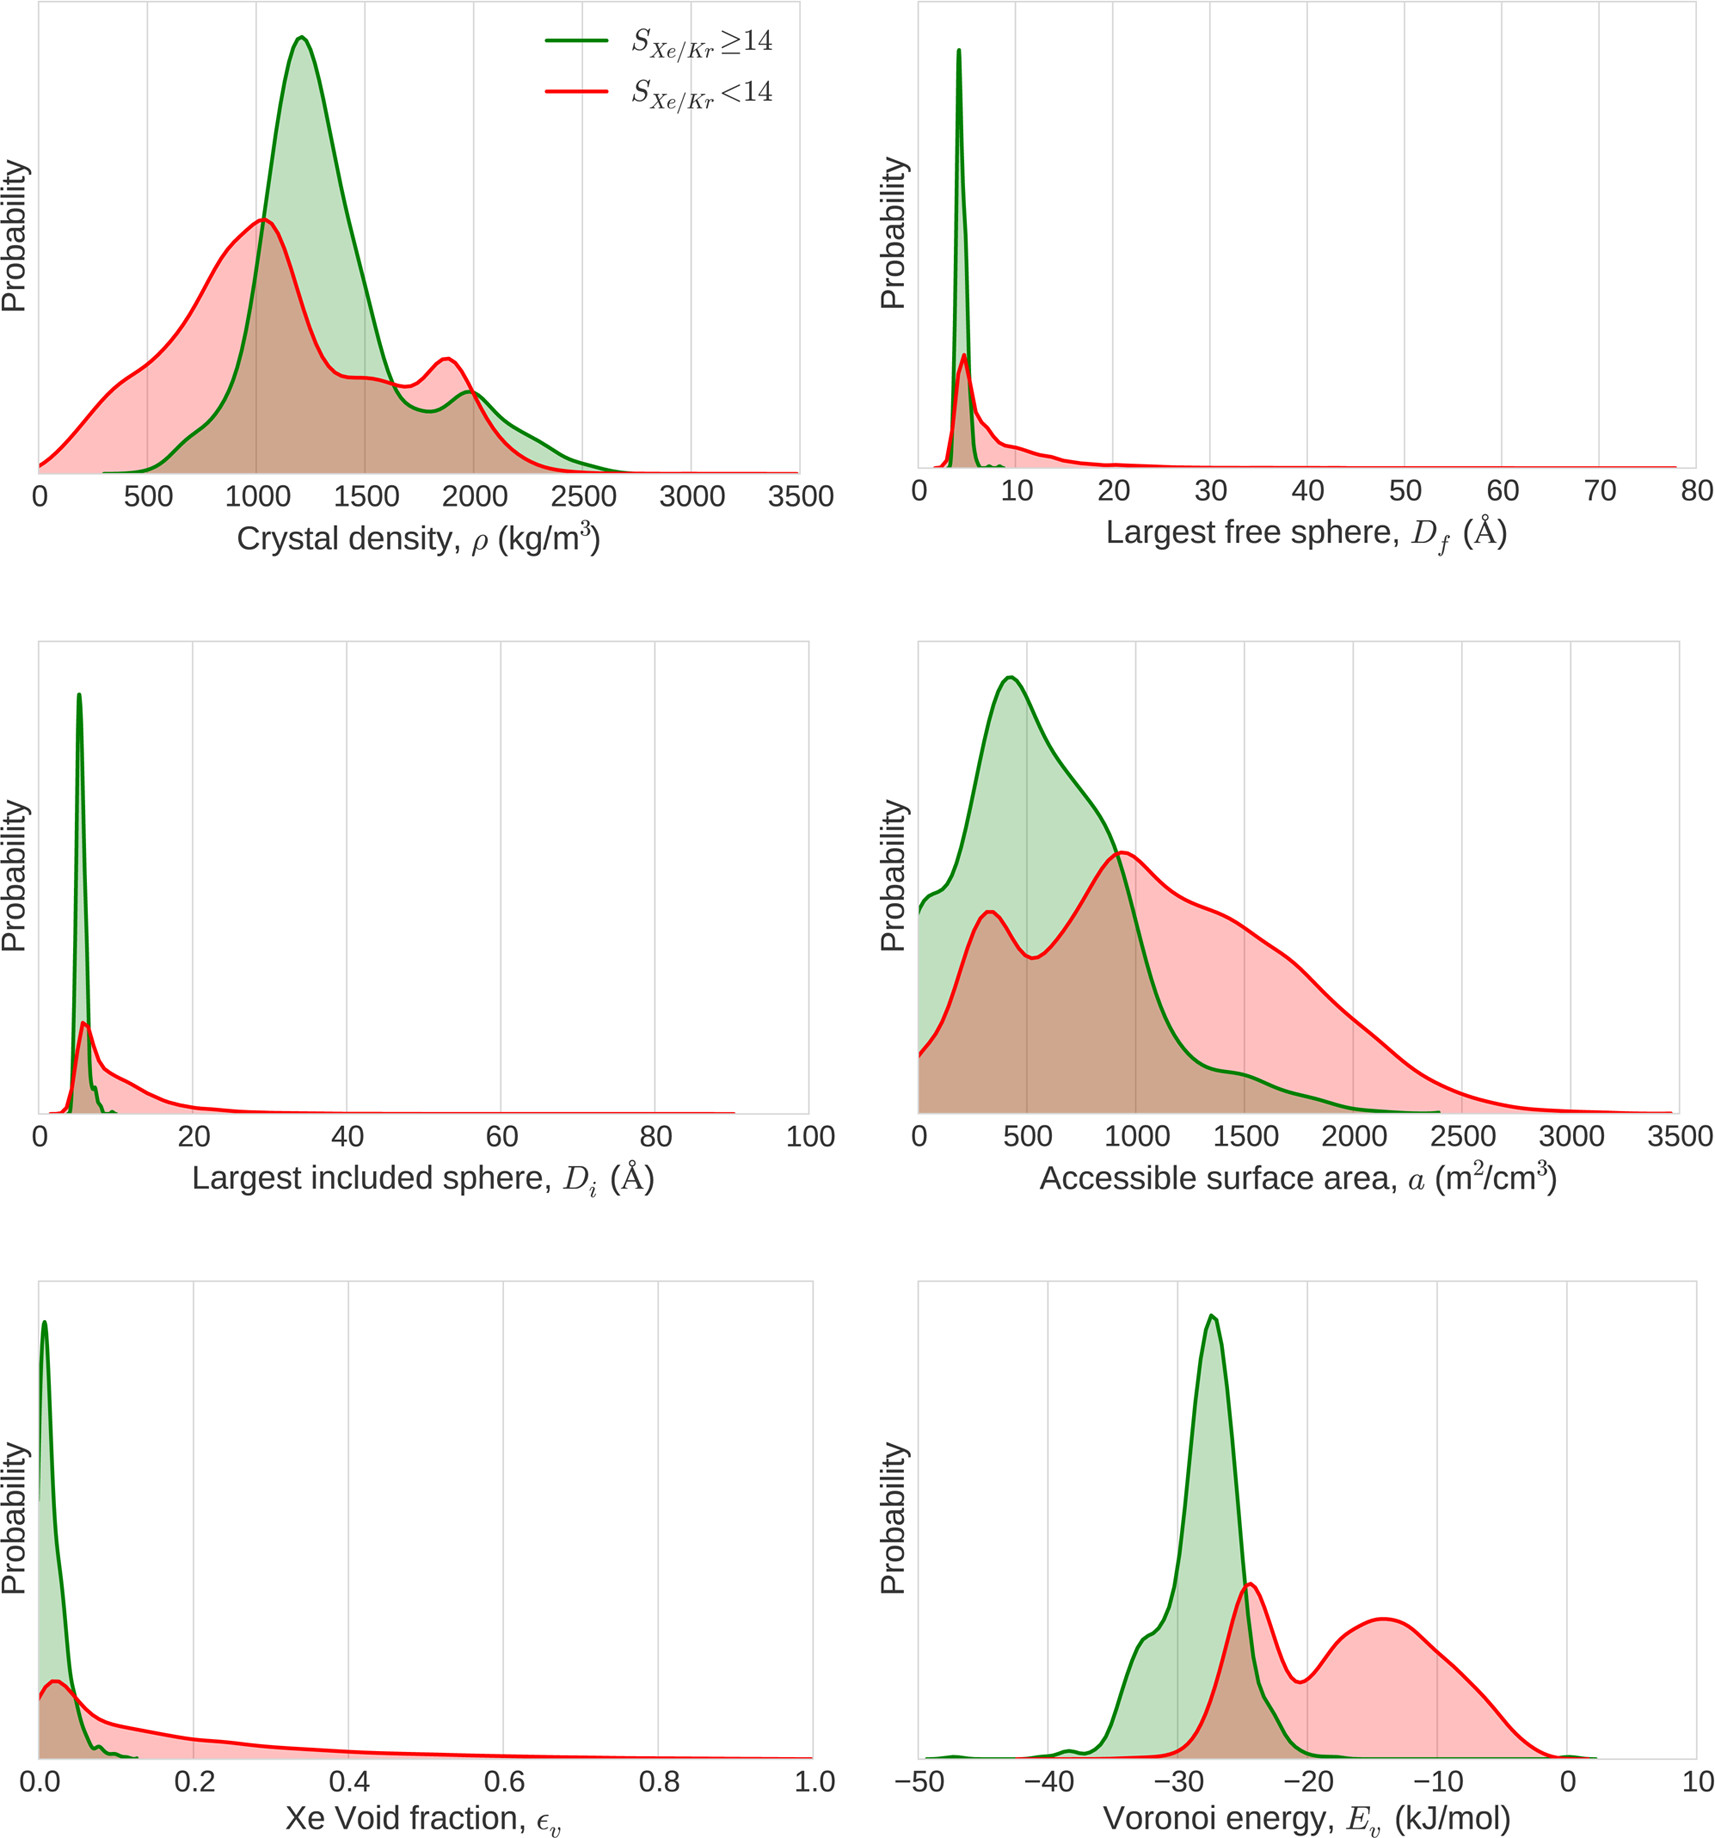
\includegraphics[width=0.7\linewidth]{figures/1-screening/Simon_2015_descriptors.jpeg}
  \caption{Statistical analysis of the adsorption separation of xenon/krypton mixtures by nanoporous materials. The graphs represent the distributions of structural descriptors explored by highly selective (green) and poorly selective (red) materials separately. Reprinted with permission from Ref.~\citenum{Simon_2015}. Copyright 2015 American Chemical Society.}
  \label{fgr:Simon2015}
\end{figure}

The experimental work on Xe/Kr separation on SBMOF-1 revealed discrepancies between the selectivity values obtained experimentally and computationally.\cite{Banerjee_2016} {The assumption of rigid crystal structures in the molecular simulations could partially explain the difference observed.} Witman et al.\ proposed that the flexibility of the materials, that weren't considered in the screening of Simon et al., could explain the lower selectivity observed experimentally.\cite{Witman_2017} In this study, they screened the Henry regime separation of about 4,000 MOF structures of the CoRE MOF 2014 database\cite{Chung_2014}, and found that intrinsic flexibility, i.e.\ the thermal vibration of the material, can make the pore size derive from the ideal value for the separation and hence lower the selectivity. This study further confirms the importance of the pore size by highlighting the effect of its evolution over time.

In 2019, Chung et al.\ screened the most extensive simulation-ready and experimentally synthesized MOF structures for Xe/Kr separation.\cite{Chung_2019} This study pointed out the potential of coordinated solvent molecules to fine-tune the selectivity for any separation application, since their presence can enhance selectivity in some cases. The results of their screening confirm the potential of structures such as SBMOF-1 found by Simon et al., but they also described a few structures with similar selectivity but with better xenon uptake. The authors emphasize the importance of considering other figures of merit such as the adsorption capacity. Other factors should be taken into account to find the best trade-off between all the relevant figures of merit; we could think of the kinetics of such a separation, the effect of flexibility on the performance, the stability of the materials (especially in radioactive environment), the financial aspects, and more.

After this quick overview of the different screening studies in the field of xenon/krypton separation, we are now going to detail its industrial context, the foreseen top materials that could fulfill the industrial separation and what further studies are needed to better understand the process while discovering new materials.


\section{Xenon/krypton separation}

In this section, we will try to see how we can apply the above-mentioned screening methodologies to help us understand the origins of the Xe/Kr separation and identify promising materials for industrial applications. 

\subsection{Industrial applications}


The industrial interest for noble gases lies first and foremost in the many applications attached to them. For instance, xenon has multiple applications in the medical (e.g.\ anesthesia, painkiller, imaging),\cite{cullen1951anesthetic, holstrater2011intranasal,Mammarappallil_2019} aeronautical\cite{Patterson_2002,Coxhill_2005}, lithographic\cite{Abramov_2018}, microelectronic\cite{Chang_1995} or lighting sectors,\cite{Jarman_1974,Tanaka_2019} just to cite a few. To meet the demand for these noble gases, one should consider all available sources, the most obvious one being the air we breathe. Xenon and krypton have both very low atmospheric concentrations; out of a thousand liters of air we would extract at most one-tenth of a milliliter of xenon and one of krypton.\cite{kerry2007industrial} Nevertheless, direct extraction from the air remains the main production mean for xenon and krypton along with chemical plant off-gases that contains a higher concentration of inert gas (e.g. amonia purge gas). In these cases, the industry more commonly uses cryogenic distillation to extract xenon and krypton, which requires a compression and cooling of the gas mixture at very low temperatures. The separation process can be broken down into three steps: first the condensation of all gas with a boiling point higher than the oxygen, then the purification of oxygen resulting in a 20-80 xenon/krypton mixture, and finally the separation of xenon from krypton. In 1997, several cases of explosion of separation units were caused by the reaction of non-filtered dangerous hydrocarbons with purified liquid oxygen produced in the second step of this long process.\cite{distill_accident,distill_accident2} The extreme chemical and physical conditions required for cryogenic distillation support the need for less energy-intensive and safer alternatives. 

The role of a dispatchable source of low-carbon energy can only be fulfilled by batteries charged by renewable energies (wind or solar) or by nuclear plants. However, one of the major criticisms on this source of energy concerns the management of the radioactive waste. As promising technologies in gas separation emerge, there is an increasing need for a solution for the release of very small amount of radioactive off-gases like Kr\e{85} from nuclear spent fuels.\cite{Blomeke_1969} Furthermore, stable xenon isotopes are also produced in these spent nuclear fuels, which can be used in all the above-mentioned applications. In the context of a regained interest in nuclear energy, the fourth generation nuclear plants are projected to be built on other technologies such as the light water or the molten salt technologies.\cite{LeBlanc_2010} Molten salt reactors would continuously produce xenon and radioactive krypton in the electricity generation process.\cite{Riley_2019} The development of gas separation units in these facilities would represent a promising source for xenon production. Yet, we can laboriously imagine deploying standard cryogenic distillation units in a nuclear facility for obvious security reasons. Consequently, nanoporous materials are considered as the alternative technology for xenon/krypton separation. Zeolites are already used as a pre-purification system,\cite{kerry2007industrial} and they are now projected to be used as a standalone separation system. 

\begin{figure}[ht]
  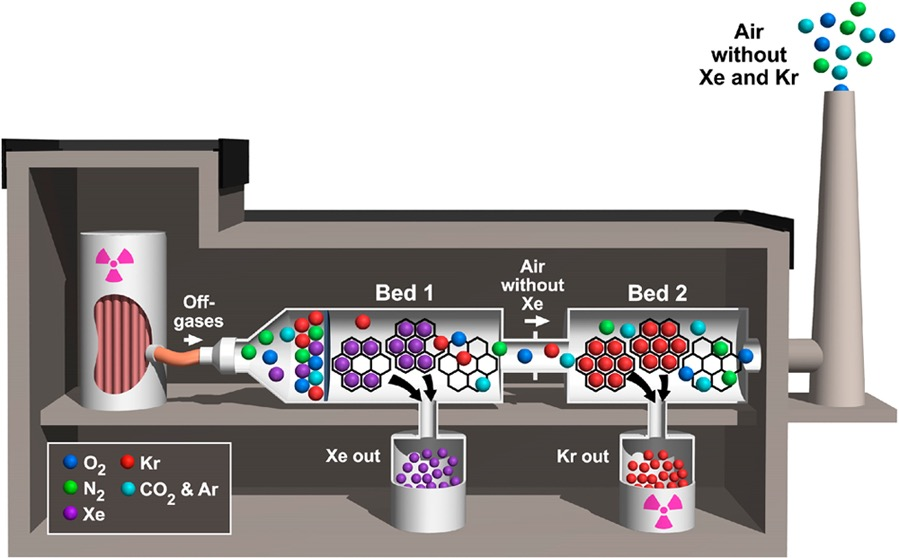
\includegraphics[width=0.49\textwidth]{figures/1-screening/Kr_treatment.jpg}
  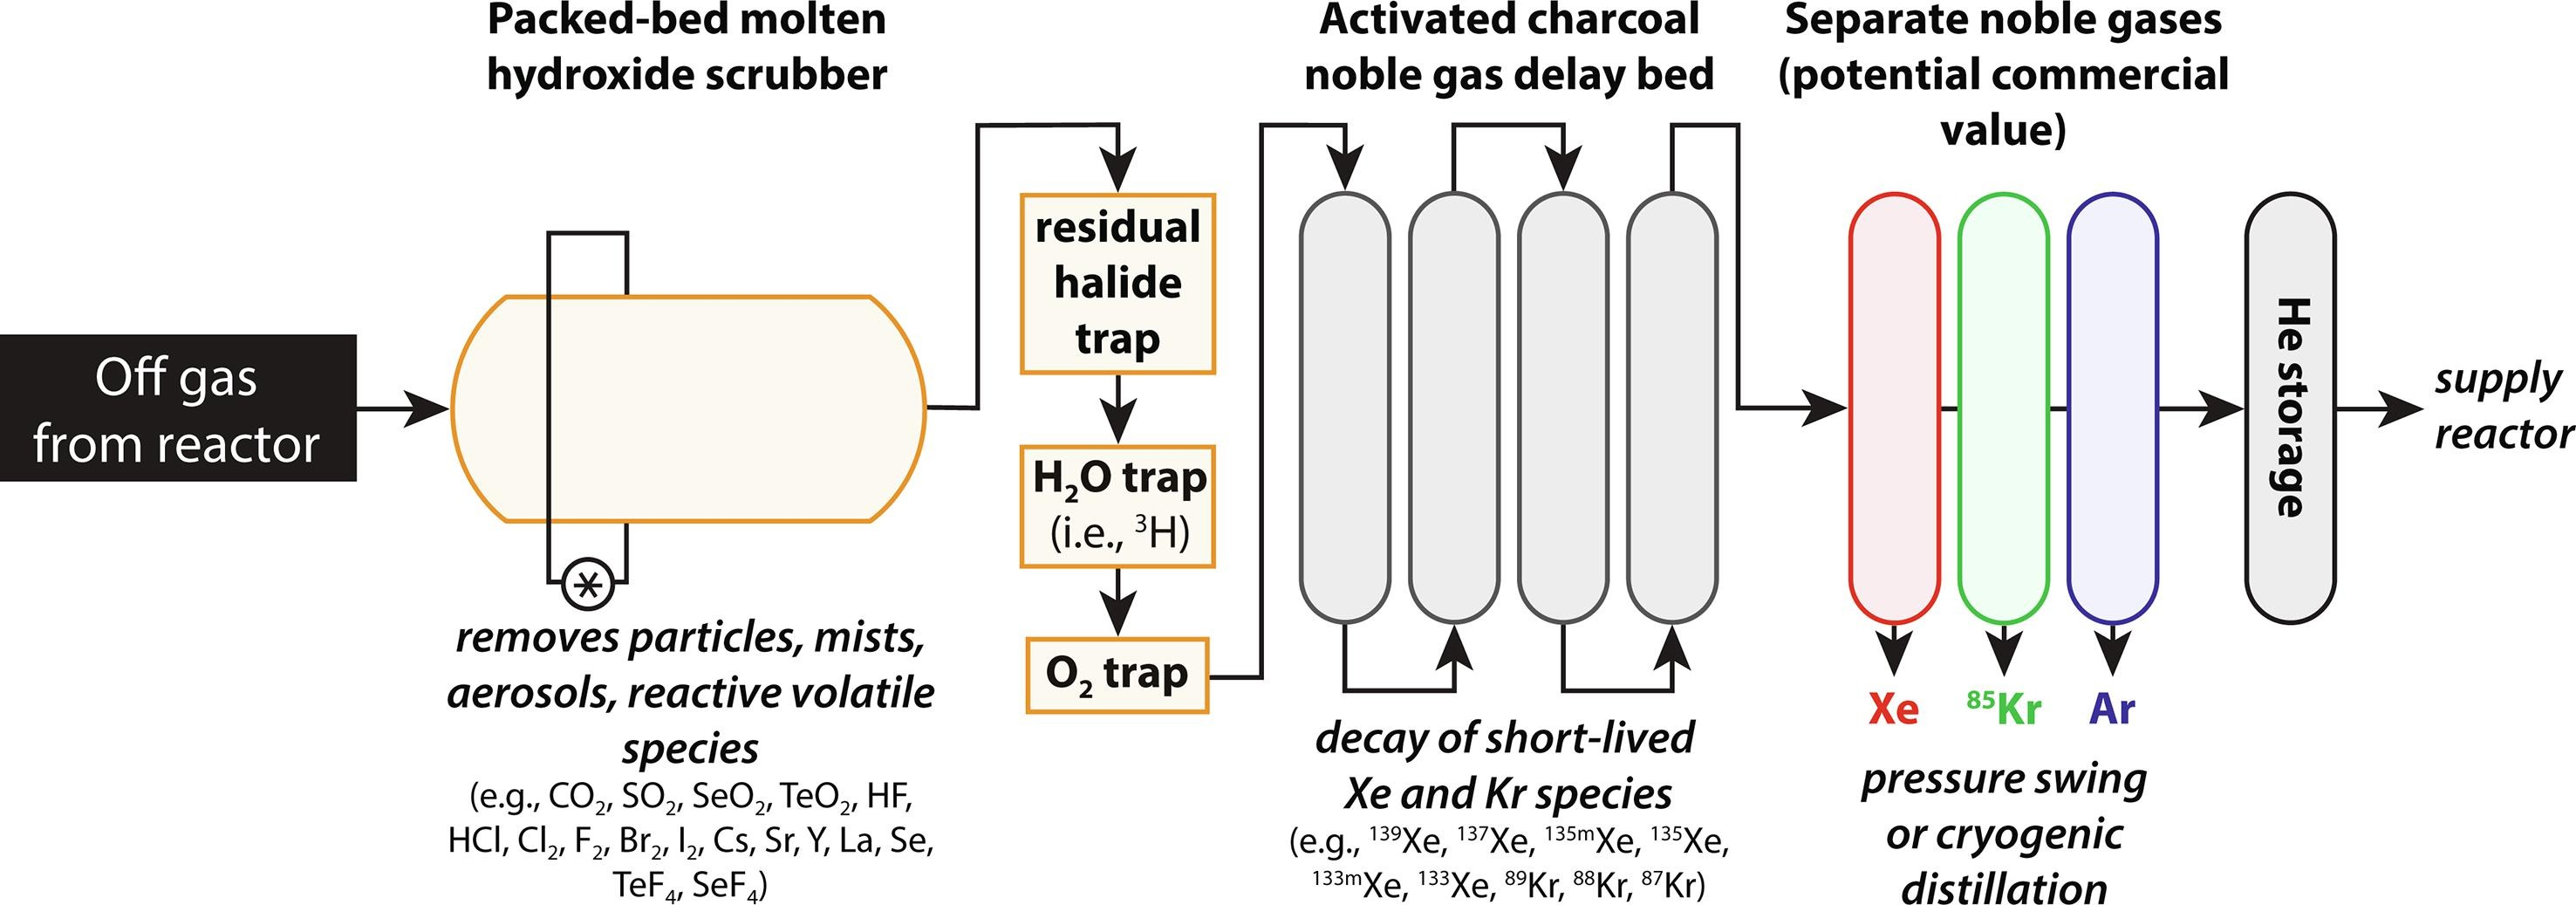
\includegraphics[width=0.49\textwidth]{figures/1-screening/MSR_noble_gas.jpg}
  \caption{Representation of xenon/krypton separation process using porous materials in a nuclear fuel reprocessing plant and in a molten salt reactor. Reprinted with permission from reference \citenum{Banerjee_2014} copyright \copyright (2014) American Chemical Society and reference \citenum{Riley_2019} copyright \copyright (2019) Elsevier.}
  \label{fgr:industrial}
\end{figure}

Banerjee et al.\ proposed a two-bed system with a first bed filled with MOFs designed for xenon separation and then a second one for radioactive krypton capture.\cite{Banerjee_2014} The authors proposed some examples of material that could be used for this separation unit; more research is needed to find out what are the best materials for these separations. In the following section, we will review the most promising materials for this separation and the structural explaining their high performance. 


\subsection{Promising Materials for the xenon/krypton Separation}

Several experimental reports used the strategy outlined by computational screenings to improve separation properties, as well as tuning the chemical nature of the organic linkers. The main criteria outlined by the different studies on xenon/krypton separation call for pore size tailor-made for xenon and also for maximized interactions with the framework atoms obtained either through the chemical nature or the shape of the cavities. 

In the early phase of the experimental design of materials for the xenon/krypton separation, Wang et al. synthesized a cobalt MOF \ce{Co3(HCOO)6} with a selectivity of 12 that present rather narrow pores (around \SI{5}{\angstrom}) connected by zig-zag segments.\cite{Wang_2014} Later, Chen et al. synthesized a selective porous cage material by not only focusing on the pore size but more importantly on the shape of the cavity, the selectivity of around $20$ was considered record high at that time. For instance, the cage windows are open for small noble gases such as krypton, whereas they close around the xenon hence maximizing the interaction.\cite{Chen_2014} Mohamed et al. also designed a material with a similar selectivity,CROFOUR-1-Ni, however the performance was now explained by the chemical nature of the chromium oxide ligands that interact more strongly with the more polarizable xenon than the krypton molecules.\cite{Mohamed_2016} Finally, Banerjee et al. tested a previously synthesized\cite{KAXQIL} MOF after it was identified through high-throughput screening\cite{Simon_2015} for its outstanding theoretical selectivity around $70$. However, experimental measurements showed that its selectivity was not exceeding the one of the previous top materials. Similar emphases were made on the ideal pore size coupled with highly attractive framework atoms.\cite{Banerjee_2016}

More recently, Li et al. proposed a rigid squarate-based MOF with ``perfect pore size'' (comparable with the kinetic diameter of Xe), and an internal pore surface decorated with very polar hydroxyl groups. This material experimentally demonstrated record-high Xe/Kr selectivity of $60.6$ at low pressure (\SI{0.2}{\bar}) and ambient temperature.\cite{Li_2019} Later, Pei et al. discovered even better performing materials with Xe/Kr selectivity of $74.1$ and $103.4$ in the same conditions \SI{0.2}{\bar} and \SI{298}{\kelvin}. In addition to the perfectly tailored pore size, the structure features two oppositely adjacent open metal sites that strongly clamp the adsorbed xenon molecule.\cite{Pei_2022} These studies clearly show the potential of polar sites that preferentially interact with the more polarizable xenon over the krypton, hence explaining these record-breaking separation performances. 

\subsection{From the computer to the test tube: a rare use case}

To connect back our study to computational screenings, we are now going to present one of the rare cases of direct contribution of high-throughput screenings to the lab testing of a material. In 2015, Simon et al.\cite{Simon_2015} analyzed the Nanoporous Materials Genome,\cite{Simon_2015_EES, Boyd_2017} a database of about 670,000 experimental and hypothetical porous material structures, including MOFs, zeolites, PPNs, ZIFs, and COFs, for candidate adsorbents for xenon/krypton separations. This study led to the rediscovery of SBMOF-1, a promising nanoporous material that was presented one year later.\cite{Banerjee_2016}

It is possibly the largest-scale study performed in this area, both by the sheer number of frameworks involved and by the diversity of their nature. Because such a set is too big for brute-force screening with GCMC simulations, they proposed a multiscale modeling strategy combining machine learning algorithms (trained on a diverse subset of 15,000 materials) with molecular simulations (used both to generate the ML training data, and to refine the separation properties for the top performers obtained by the ML predictor). Without going into details (see Fig.~\ref{fgr:Simon} for more details), the ML model they trained was mainly based on geometric structural descriptors, with the addition of a single energy-based descriptor: the Voronoi energy\ (i.e.\ the average energy\ of a xenon atom at the accessible nodes in the Voronoi partition of space). In addition to identifying and describing some top performing materials, the authors also analyzed the correlations between high Xe/Kr selectivity and the geometric properties of the frameworks, in order to ``rationalize the strong link between pore size and selectivity''. In particular, by developing theoretical pore models of spherical and cylindrical geometries, they could highlight the general geometrical trends observed, but also the fact that there is a wide diversity of performance beyond the geometrical features of the frameworks, which suggests the key role of the chemical nature of the cavities.

\begin{figure*}[t]
    \centering
    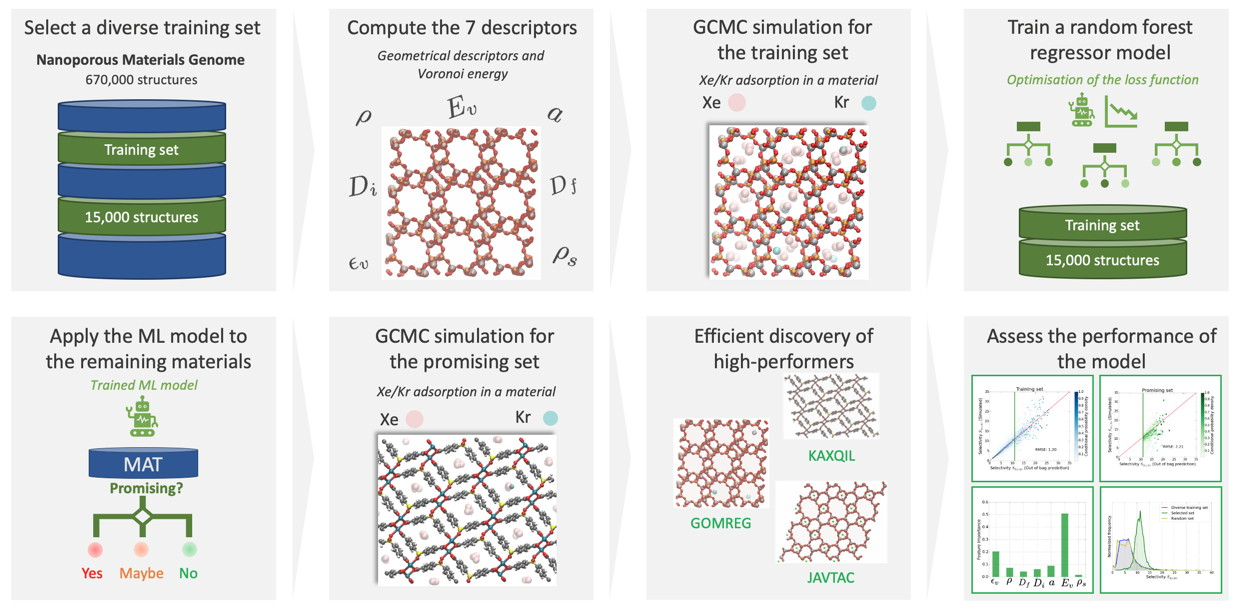
\includegraphics[width=0.98\textwidth]{figures/1-screening/Simon.jpg}
    \caption{\ Schematic representation of large-scale screening of nanoporous materials for Xe/Kr adsorption-based separation by Simon et al.,\cite{Simon_2015} based on a combination of Grand Canonical Monte Carlo simulations and machine learning algorithm (Random Forest Regressor). The main goal of this screening is to find high-performing materials in a large dataset of both experimental and hypothetical materials. 
    Adapted with permission from Ref.~\citenum{Simon_2015}. Copyright 2015 American Chemical Society.
    }\label{fgr:Simon}
\end{figure*}

The chemical nature of the cavities was best described using the Voronoi energy descriptor they developed. This descriptor gives an idea of the xenon adsorption isosteric heat of the material. Given these results, more studies should focus on describing the adsorption thermodynamic quantities such as the adsorption enthalpy but also the Henry adsorption constants. This study finally leads to the synthesis and testing of one of the top performing materials in the field. However, we cannot stop but wondering why there is a discrepancy between the theoretical selectivity of around $70$ of SBMOF-1 and its actual experimental selectivity of $16$. In the final chapter of this thesis, we will try to give an explanation for this. In the future, such close collaboration between experimental and computational teams are crucial even if they are still too rare. A recent paper suggests that these collaborations are rare across all nanoporous fields and a lot of improvements are needed to foster cooperation between the labs.\cite{Li_2022}


\subsection{The Future of Screening}

%flexibility
Despite the progress made, important drawbacks of the current methodologies remain. High-throughput screenings rely too much on oversimplified assumptions such as the rigidity of the framework, the absence of defects, the use of Lennard-Jones potentials and inaccurate charges. For instance, the rigidity of the framework only takes into account one conformation of the framework. Yet, thermal agitation induces a ``breathing'' movement of the framework with an amplitude dependent on its intrinsic flexibility. The pores of the framework can change depending on the number of adsorbates to interact more optimally with them, which can be induced by a change in pressure. The issue of flexibility is rarely tackled, and when considered, it is only on the few most selective structures given by an inaccurate screening based on the rigid crystal approximation. One can wonder about the results obtained if it is applied to larger sets of structures. Witman et al.\ found that flexibility applied to top performing materials can decrease the selectivity, because the pore does not have an optimal size anymore.\cite{Witman_2017} In some cases, the selectivity of a well-performing material can even increase to become a top performing one. Computational screenings can be closer to predict experimental values of selectivity, diffusivity, and other key performance metrics.

%Diffusion
Many open problems remain for the design of efficient high-throughput computational screenings. The connection between different properties for a given application is not systematically integrated in the screening procedures. For example, in methane storage, the working capacity of the material is the main property to optimize, but the kinetics of the adsorption/desorption or the mechanical resistance to compaction among others also need to be considered. Designing a nanoporous material is in fact a multivariate optimization problem with tacit constraints, for example the {synthesizability}. For instance, the diffusion coefficients of adsorbates in a xenon/krypton separation problem can help us better understand the breakthrough simulations and eventually the whole separation process in pressure or temperature swing adsorption beds. For this reason, studying transport properties along with uptake capacities and thermodynamic selectivity of the xenon/krypton separation can give a more complete picture of the industrial process we ultimately want to model. 

%Polarization
Moreover, the transferability of the methodology to a broad range of materials is often achieved at the expense of accuracy in specific cases. And one can rightly question the universality of depending on faster but less elaborated models, which boils down to a trade-off problem between prediction accuracy and computational cost (or complexity). For instance, classical forcefields are broadly used in rigid materials for adsorption properties, but the switch to more costly \emph{ab initio} methods or the addition of flexibility can result in a more accurate description at the expense of computational resources. The addition of polarization could be very promising since several top performing materials harbor open metal sites and highly polar sites that explain the acute affinity to xenon adsorbates. 

% ML
The development of ML-assisted screenings is paired with the advances in data science techniques and algorithms. Recent advances in deep learning have enabled the development of transformer-based (the technology at the base of ChatGPT for example) machine learning models to predict adsorption properties.\cite{Kang_2023,Cao_2023} More importantly, the construction of descriptors tailored to the many possible applications is also an ongoing work. This construction work cannot be dissociated to the physical and chemical intuition of the scientists. Topological, chemical, electronic and other descriptors have been developed on top of the more common geometrical and thermodynamic descriptors, which displays the importance of strong physical chemistry knowledge. Recently Shi et al.\ highlighted the key role of energy histograms in predicting adsorption properties.\cite{Shi_2023}
The discovery of novel relevant descriptors remains the main lever for increased performance of the ML models and is closely related to a rigorous theoretical work.
For these reasons, we worked during this thesis on more accurate and faster ways of calculating these interaction energies to extract valuable energy/thermodynamic descriptors.


The development of databases is another key aspect in the promotion of data science in the field of materials science in general, and nanoporous materials chemistry in particular. The diversity of materials, the inclusion of experimental data (successful or failed), the addition of under-studied classes of materials (e.g.\ amorphous) are all key aspects to upgrade the existing database. Even if existing attempts to create a centralized database have been initiated by the materials project,\cite{MaterialsProject} this database does not contain all the existing information on each material. Furthermore, this high amount of data will need to be efficiently explored, and non-supervise deep learning algorithms have been developed to do so.\cite{Park_2023} Coupled with synthesis robot, these methods can navigate through the unexplored databases to find the few most interesting candidates for a given targeted application.

In the future, computational high-throughput screening could be integrated more tightly into the design process of nanoporous materials, hence further improving its efficiency. The computational prescreening can be coupled with automated screenings of the most promising materials to finally identify candidates for further studies. This automated design process is described by Lyu et al.\ in their paper on ``Digital Reticular Chemistry'' and set out promising perspectives for computational screenings in the field.\cite{Lyu_2020} Some studies are already pioneering this new research area by combining high-throughput characterizations, active learning algorithms and robotic synthesis.\cite{Greenaway_2018,Moosavi_2019} Another step towards faster industrialization would integrate process modeling to enrich the purely atomistic approach.

\OnlyInSubfile{\printglobalbibliography}

\end{document}
